\section{Rozpoznávanie tváre}\label{l:techn}
V tejto časti práce sa budeme venovať problematike rozpoznávania tváre, popíšeme ako je možné rozdeliť rozpoznávanie tváre z pohľadu porovnávania,
ukážeme z akých krokov vo všeobecnosti pozostáva proces rozpoznávania tváre a nakoniec popíšeme niektoré známe techniky používané pri rozpoznávaní tváre. \\

\indent Rozpoznávanie tváre je jedným z úkonov, ktoré človek robí pravidelne a bez námahy v každodennom živote.
Široká dostupnosť silných počítačov za nízku cenu vytvára obrovský záujem o automatické spracovanie digitálneho
obrazu v širokom spektre aplikácií, ako sú napríklad biometrická autentifikácia, monitorovanie osôb,
interakcia s počítačom či spravovanie multimédií.
Výskum a vývoj v oblasti rozpoznávania tvárí nasleduje tento trend
automaticky.\\
\indent Hlavnými výhodami využívania rozpoznávania tvárí voči iným biometrickým metódam ako napríklad odtlačky prstov či dúhovka,
je ich prirodzené a nerušivé používanie, ale najmä možnosť použitia na väčšiu vzdialenosť. Zo šiestich biometrických metód(tvár, odtlačky prstov, dlaň, hlas, dúhovka, podpis)
je podľa The International Civil Aviation Organization(ICAO)\cite{icao} rozpoznávanie tváre primárnou metódou pri kontrole identity na letisku.\\
\indent Prvým automatickým systémov na rozpoznávanie tvárí bol podľa\cite{handbookface}, systém navrhnutý Takeo Kanadem v jeho práci\cite{kanade1974} z roku 1974.
Za ním nasledovalo obdobie bez výraznejšieho pokroku v automatickom rozpoznávaní tváre, až do roku 1990, kedy Sirovich a Kirby zverejnili článok\cite{kirby1990application},
v ktorom popisujú využitie nízko-dimenzionálnych reprezentácií tváre odvodenej z Karhunen-Loevovej transformácie alebo Principal Component Analysis(\acrshort{pca}).
Podľa Jaina v\cite{handbookface} bol ďalším veľkým míľnikom práca\cite{turk1991eigenfaces} od Turka a Pentlanda na vlastných vektorov tváre(eigenface),
ktorá znovu naštartovala výskum v oblasti rozpoznávania tváre. Medzi ďalšie míľniky tiež Jain zaraďuje prácu na Fisherovej metódae\cite{belhumeur1997eigenfaces},
ktorá aplikuje Linear Discriminant Analysis(LDA) po aplikovaní PCA k dosiahnutiu vyššej presnosti, výskum na lokálnych Gaborových filtroch\cite{wiskott1997face}
k dosiahnutiu efektívnejších príznakov tváre a prístup AdaBoost učenia, založeného na architektúra kaskádneho klasifikátora pre detekciu v reálnom čase\cite{viola2001rapid}.\\
\indent Od obdobia kedy bola narhnutá Eigenface metóda nastal veľký pokrok v oblasti rozpoznávania tváre.
V kontrolovaných podmienkach, kde je možné ovládať svetelnosť,
postoj osoby či výraz tváre, prekonáva automatické rozpoznávania tváre ľudí, a to najmä pokiaľ databáza obsahuje veľké množstvo snímkov tváre.
Napriek tomu rozpoznávanie tváre
stále čelí mnohým výzvam, najmä problematike rozpoznávania tváre v neriadených podmienkach.

\subsection{Rozdelenie}
Ako aj ostatné biometrické systémy, aj rozpoznávanie tváre funguje v jednom alebo oboch z režimov:

\begin{itemize}
	\item Verifikácia(autentifikácia)
	\item Identifikácia tváre
\end{itemize}

Pri verifikácii tváre ide o porovnanie jedna k jednej, čo znamená, že jeden snímok tváre sa porovnáva len jedným záznamom identity v databáze, za ktorú sa prehlasuje.
Typickým využitím tohoto režimu je samoobslužná kontrola identity prostredníctvom elektronického pasu\cite{handbookface}.\\
\indent Identifikácia tváre zahŕňa porovnanie jedna k mnohým, čo znamená, že jeden snímok tváre sa porovnáva s viacerými záznamami identít v databáze a vyberie jednu\cite{handbookface}.
V niektorých prípadoch využitia je postačujúce nájsť len najpodobnejšiu identitu.
V iných prípadoch, ako napríklad sledovanie podozrivých osôb,
je okrem nájdenia najpodobnejšej tváre potrebné zaviesť aj prah spoľahlivosti, a tie tváre ktoré dosiahli mieru podobnosti väčšiu ako je prah, sú zaznamenané.\\
\indent Úspešnosť systému na rozpoznávanie tváre závisí vo veľkej miere na množstve variabilných faktorov, ako je osvetlenie, poloha tváre, mimika, vek, make-up, účes,
brada či pohyb tváre. Na základe týchto faktorov Jain rozdeľuje\cite{handbookface} na 2 kategórie vzhľadom na miery spolupráce užívateľov:

\begin{itemize}
	\item Scenár so spolupracujúcim užívateľom
	\item Scenár s nespolupracujúcim užívateľom
\end{itemize}

\indent Prípad spolupracujúceho užívateľa je využívaný napríklad pri prihlasovaní do počítača, riadenie fyzického prístupu, elektronické pasy(e-passport), teda prípady kedy má
užívateľ záujem spolupracovať na správnom zosnímaní tváre(pod správnym zosnímaním tváre môžeme rozumieť napríklad snímok tváre z predu s neutrálnym výrazom a otvorenými očami)
kvôli prístupu alebo povoleniu.\\
\indent V prípade nespolupracujúceho užívateľa, ktorý je typické pre už spomínané sledovanie podozrivých, si osoba nie je vedomá toho, že podlieha identifikácii.
Čo sa týka vzdialenosti
medzi tvárou osoby a kamerou, sa v spolupracujúcom scenári využíva krátka vzdialenosť, typicky o jedného metra, a ide teda o oveľa jednoduchšiu úlohu v porovnaní s identifikáciou
nespolupracujúcej osoby často na väčšiu vzdialenosť.

\subsection{Proces identifikácie}
Jain popisuje rozpoznávanie tváre takto: ``Rozpoznávanie tváre sa zaraďuje medzi problémy rozpoznávania vzorov, kde tvár, ktorá je reprezentovaná ako trojrozmerný objekt,
podlieha odlišnostiam vo svetle, postoji, výraze a iných faktoroch, potrebuje byt identifikovaná na základe zozbieraných obrázkov``\cite{handbookface}.
Zatiaľ čo rozpoznávanie tváre z dvojrozmerného snímku je dnes bežne používané vo vačšine prípadov, v niektorých, najmä tých, ktoré vyžadujú vyššiu bezpečnosť,
sa využíva trojrozmerný snímok tváre,
prípadne snímky tváre mimo bežne viditeľného spektra - napr. termografický snímok tváre.  Systém na rozpoznávanie tváre sa podľa Jaina\cite{handbookface} vo všeobecnosti skladá zo štyroch
základných častí, ako je ukázané na obrázku\ref{fig:workflow}:

\begin{itemize}
	\item Detekcia tváre a lokalizácia vváre
	\item Normalizácia tváre
	\item Extrakcia príznakov
	\item Hľadanie zhody tváre
\end{itemize}

\begin{figure}[H]
	\centering
	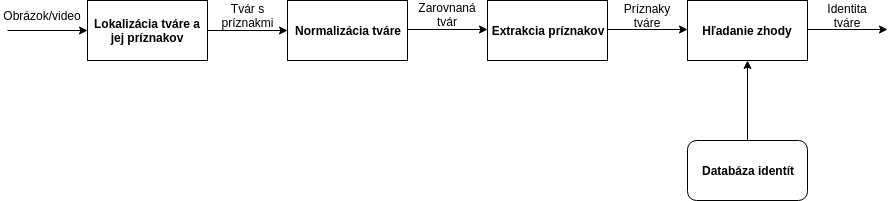
\includegraphics[width=1\linewidth]{img/workflow}
	\caption{Proces rozpoznávania tváre}
	\label{fig:workflow}
\end{figure}

\indent  Pri detekcií tváre ide primárne o oddelenie oblasti tváre od pozadia snímku.
V prípade videa je potrebné sledovať(track) detekovanú tvár naprieč niekoľkými snímkami videa pomocou komponentu na sledovanie pohybu tváre.
Zatiaľ čo detekcia tváre poskytuje len hruby odhad polohy a veľkosti tváre, lokalizácia bodov tváre najde už konkrétne časti tváre,
ako sú napríklad oči, nos, obrys tváre a podobne.
Lokalizácia bodov tváre je zväčša vykonávaná osobitným komponentom na lokalizáciu bodov alebo komponentom na vyrovnanie(alignment) tváre.\\
Normalizácia tváre ide o normalizáciu tváre v geometrickom a fotometrickom zmysle.
Tento krok je nevyhnutný, pretože sa od najnovších a najlepších(state-of-the-art) rozpoznávacích metód očakáva, že dokážu rozpoznať tvár v rôznych polohách a rôznom svetle.
Geometrická normalizácia vykonáva transformáciu tváre do štandartného formátu snímku pomocou orezania(crop) tváre \cite{handbookface}.
Snímok je následne zakrivený(warp) a upravený(morph) kvôli ešte lepšej a presnejšej normalizácií tváre \cite{handbookface}.
Úlohou fotometrickej normalizácie je spracovanie snímku na základe osvetlenie či farebnej škály.\\

\indent Extrakcia príznakov je vykonávaná na normalizovanom snímku tváre, s cieľom vybrať charakteristické informácie, ktoré sú užitočné pri rozlišovaní tvárí rozdielnych osôb,
pričom odolný voči odchýlkam v geometrickej a fotometrickej normalizácii \cite{handbookface}.
Extrahované príznaky sú následne použité pri hľadaní zhody s identitou.\\

\indent Pri hľadaní zhody tváre sa porovnávajú extrahované príznaky zo vstupnej tváre s jednou alebo viacerými tvárami ktoré už sú zapísané v databáze.
Výsledkom porovnania s jednou tvárou je výsledkom odpoveď áno alebo nie(verifikácia).
V prípade porovnávania s viacerými tvárami je výsledkom identita vstupnej tváre, za predpokladu, že identita ktorá je nájdená presiahne prah spoľahlivosti,
inak vráti informáciu, že tvár je neznáma.
V súčastnosti je v tejto oblasti najväčšou výzvou nájsť spoľahlivé meranie vhodné na určenie podobnosti príznakov tváre.\\
\indent Presnosť systému na rozoznávanie tváre vo veľkom závisí na správnosti extrahovaných príznakov tváre, ktoré zase závisia od správnej lokalizácii a normalizácii tváre.

\subsection{Techniky rozpoznávania tvári}
Zhao rozdeľuje\cite{zhao2003face} algoritmy rozpoznávania do dvoch základných kategórií, vzhľadom na spôsob extrakcie príznakov:

\begin{itemize}
	\item Metódy založené na príznakoch(feature-based)
	\item Medódy založené na vzhľade(appearance-based)
\end{itemize}

Metódy založené na príznakoch využívajú rôzne vlastnosti a geometrické atribúty na popis tváre, ako sú napríklad vzdialenosti či uhly medzi bodmi tváre.
Na druhej strane, metódy založené na vhľade využívajú globálne vlastnosti tvárového vzoru.
Typickou črtou algoritmov založených na vhľade je výpočet bázových vektorov, na ktoré je následne tvár premietnutá.
Koeficienty takejto projekcie sú potom použité k efektívnej reprezentácii údajov tváre\cite{handbookbio}.
Obľúbené algoritmy ako sú Principal Component Analysis(\acrshort{pca}), Linear Discriminant Analysis(\acrshort{lda}), Indenpendent Component Analysis(\acrshort{ica}),
Local Feature Analysis(\acrshort{lfa}), Manifolds, Correlation Filters alebo Tensorfaces sú založené práve na vhľade tváre.
Holistický prístup k rozpoznávaniu tváre má však často problémy pri rôznych polohách tváre\cite{handbookbio}.

\subsubsection{Eigenfaces}
Podstatou metódy Eigenfaces navrhnutej Turkom a Pentlandom\cite{turk1991eigenfaces}, tiež známej ako PCA,
je hľadanie najmenšej kvadratickej chyby lineárneho podpriestoru,
ktorý mapuje dáta z originálneho N-rozmerného priestoru na M-rozmerný priestor príznakov, kde M << N .
Týmto dosiahneme redukciu dát do M-rozmerného priestoru využitím M vlastných vektorov matice kovariance, ktoré korešpondujú s najväčšími hodnotami vlastných čísel\cite{handbookbio}.
Konečné bázové vektory ktoré sú najvhodnejšie na popis dát, sú nájdené pri procese optimalizácie, ktorej podstatou je  maximalizácia variancie premietnutých dát.
Jain popisuje\cite{handbookbio} proces výberu bázových PCA vektorov W optimalizačnou funkciou\eqref{eqn:pca}, kde S\textsubscript{T} označuje úplne maticu rozptylu,
ktorá obsahuje kovariancie dát tváre.


\begin{equation}\label{eqn:pca}
	W_{PCA} = arg max|W^T S_T W| = [w, w2,\dots,wm]
\end{equation}

\begin{figure}[H]
	\centering
	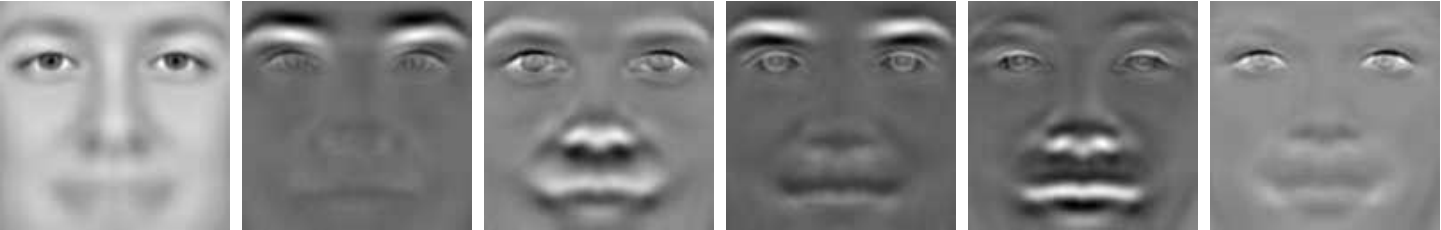
\includegraphics[width=1\linewidth]{img/eigenfaces}
	\caption{Prvých 6 bázových vektorov Eigenfaces, té z\cite[s.~45]{handbookbio}}
	\label{fig:eigenfaces}
\end{figure}

Na obrázku\ref{fig:eigenfaces} vidíme príklad vlastných vektorov vybraných metódou Eigenfaces, na obrázkoch po procese normalizácie.
Metóda PCA je vhodná na reprezentáciu dát, čo neznamená, že je vhodná aj na rozdeľovanie do tried.

\subsubsection{Linear Discriminant Analysis, Fisherfaces}
Matóda LDA\cite{duda2012pattern} je oveľa vhodnejšia k hľadaniu projekcií, ktoré dobre oddeľujú rozdielne triedy.
Táto metóda je založená na hľadaní optimálnych projekčných vektorov, ktoré optimalizujú pomer medzitriednych(within class) a vnútrotriednych(between class) vzdialeností - maximalizuje oddelenie tried
v premietnutom priestore.
Optimálne bázové vektory LDA, môžu byť podľa\cite{handbookbio} definované ako rovnica\eqref{eqn:lda}, kde S\textsubscript{B} značí medzitriednu maticu rozptylu a kde S\textsubscript{W}
vnútrotriednu maticu rozptylu.\\
\indent
\begin{equation}\label{eqn:lda}
	W_{LDA} = arg max \frac{|W^T S_B W|}{|W^T S_W W|}
\end{equation}

Zvyčajne pri riešení problematiky rozpoznávania tváre(a vačšine ostatných problémov rozpoznávania vzorov obrázkov) je množstvo tréningových obrázkov menší ako počet pixelov
(dimenzionality dát), čo znamená, že vnútrotriedová matica rozptylu S\textsubscript{W} je singulárna, čo je problémom pre LDA.
Na vyriešenie tohoto problému singulárnej matice sa na najprv vykonáva PCA na redukovanie dimenzionality dát a
až následne sa aplikuje LDA v menej rozmernom podpriestore PCA.
NA základe týchto zmien bolo dosiahnuté zlepšenie výsledkov v porovnaní s tradičnou PCA metódou.
Projekčné vektory, ktorých príklad môžeme vidiet na obrázku\ref{fig:fisherfaces}  Fisherfaces sú tie, ktorú spĺňajú maximalizujú výsledok optimalizačnej funkcie\eqref{eqn:fisher}.

\begin{figure}[H]
	\centering
	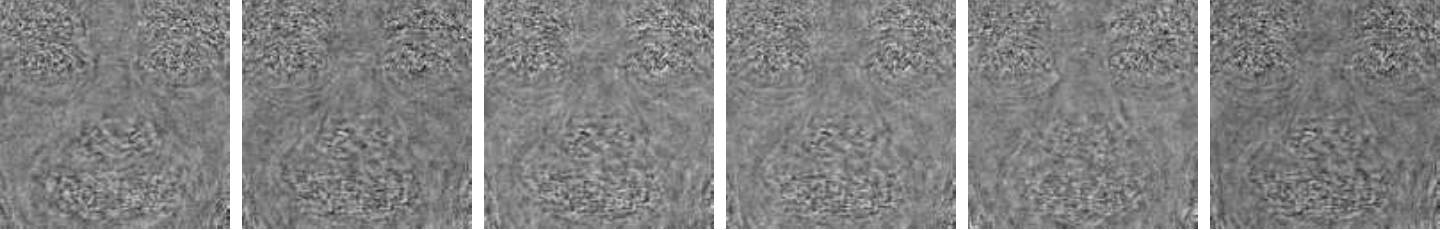
\includegraphics[width=1\linewidth]{img/fisherfaces.png}
	\caption{Prvých 6 bázových vektorov Fisherfaces, prebraté z\cite[s.~46]{handbookbio}}
	\label{fig:fisherfaces}
\end{figure}

\begin{equation}\label{eqn:fisher}
	W_{LDA} = arg max \frac{|W^T W_{PCA}^T S_B W_{PCA} W|}{|W^T W_{PCA}^T S_W W_{PCA} W|}
\end{equation}

\subsubsection{Indenpendent Component Analysis}
Podstatou metódy ICA, je hľadanie takých ne-ortogonálnych báz,
aby boli na nich založené transformácie príznakov boli štatisticky nezávislé, zatiaľ čo
metóda PCA hľadá také ortogonálne bázy tváre, aby príznaky po transformácii neboli korelované\cite{handbookbio}.
Bázové vektory tvárí metódy PCA sú založené len na štatistike druhého rádu.
ICA zovšeobecňuje koncept PCA a vytvára tak model so vzťahmi štatisticky vyššie rádu.
Pôvodná motivácia tejto metódy výchadza z potreby zaradiť zvukové vlny do nezávislých zdrojov, bez priamej znalosti procesu spájania(mixovania) týchto vĺn\cite{handbookbio}.
Bartlett vo svoje publikácií\cite{bartlett2002face}, v ktorej aplikoval metódu ICA
na rozpoznávanie tváre uvádza, že ICA dosahuje oveľa lepšie výsledky v porovnaní s metódou PCA, pri rozpoznávaní tváre v rôznych častiach dňa a rôznych výrazoch tváre.

\subsubsection{Local Feature Analysis}
LFA vytvára skupinu lokálne prepojených detektorov príznakov, založených na rozložení charakteristického podpriestoru.
Vzniknú tak minimálne kolerované a topograficky indexované podskupiny príznakov, ktoré definujú podpriestor záujmu. \cite{handbookbio} \\

\indent Lokálna reprezentácia vytvára odolnosť voči zmenám v lokalizovaných oblastiach objektov.
Príznaky použité metódoou LFA sú menej náchylné na zmenu vo svetle a zároveň je vďaka nim jednoduchšie odhadnúť
rotáciu objektu.
Algoritmus LFA bol použitý ako kľúčový komponent algoritmu FaceIt, ktorý je jedným z komerčne využívaných systémov na rozpoznávanie tváre\cite{handbookbio}.

\subsubsection{Neurónové siete a Support Vector Machines}\label{svm}
Neurónové siete(\acrshort{ns}) a Support Vector Machines(\acrshort{svm}) sú zvyčajne využívané v nízko-dimenzionálnych priestoroch príznakov, najmä kvôli výpočtovej náročnosti spracovania,
v prípade viac-dimenzionálnych dát tváre\cite{handbookbio}.
Neurónové siete podliehajú širokému záujmu o výskum, najmä čo sa týka lepšej reprezentáciu príznakov tváre a rozpoznávania tváre.
Avšak, so zvyšujúcim sa množstvom osôb, ktoré sa neurónová sieť učí rozpoznávať, narastá výpočtová zložitosť exponencionálne.
Spojením viacerých neurónových sietí sa podarilo zlepšiť celkový výkon pri rozpoznávaní tváre.\\

\indent Vo všobecnosti nevieme povedať, čo presne sa neurónová sieť naučila, alebo akým spôsobom bude fungovať.
Neurónová sieť zvyčajne vyžaduje veľké množstvo tréningových dát kvôli dobrej generalizácii dát, s čím zároveň súvisí značné množstvo výpočtov uskutočnených v procese trénovania.
SVM sa ukazuje ako úspešná metóda pri rozpoznávaní objektov, použitím kernelového triku(kernel trick), ktorý mapuje dáta do viac-dimenzionálneho priestoru príznakov\cite{handbookbio}.
SVM v tomto priestore potom nájde nadrovinu, ktorá maximalizuje šírku hranice oddeľujúcej triedy klasifikácie, a znižuje tak riziko zlej klasifikácie nielen pre trénovacie dáta,
ale tiež k dosiahnutiu lepšej generalizácie neznámych dát.\cite{handbookbio} \\

\indent Neurónovú siete v kombinácii s SVM použijeme v praktickej časti tejto práce, ktorou detekujeme príznaky tváre a následne klasifikujeme.

\newpage 

\section{Neurónové siete}\label{l:nns}
V tejto kapitole popíšeme neurónové siete, ktoré sme si zvolili ako techniku na rozpoznávanie tváre.
Začneme hlavnou stavebnou jednotkou neurónových sietí - neurónom, následne pokračujeme teóriou trénovania neurónových sietí a optimalizáciám
ako je Stochastic Gradient Descent či rôzne regularizácie.
Nakoniec tejto kapitoly popíšeme konvolučné neurónové siete a jej základné princípy, ktoré použijeme pri rozpoznávaní tváre v praktickej časti tejto práce.

\subsection{Neurón}
Základnou jednotkou z ktorej sa skladá mozog je neurón.
Kúsok mozgu, o veľkosti malého zrnka ryže, obsahuje približne 10000 neurónov, pričom každý neurón
vytvára v priemere 6000 prepojení s inými neurónmi, a ide teda v podstate o
veľkú biologickú sieť prepojení, ktorá nám dovoľuje rozumieť svetu okolo nás\cite{buduma2017fundamentals}. \\
\indent V samotnej podstate neurónu, prichádza k príjmu informácií z ostatných neurónov, 
ich spracovaniu a odoslaní výsledku spracovania ďalším bunkám.
Neurón prijíma vstupné informácií pomocou dendritov, čo sú v výbežky na konči neurónu ktoré sa správajú ako 
ako antény a zachytávajú signály.
Každé z týchto prepojení je dynamicky zosilnené alebo zoslabené, závislosti od frekvencie používania daného spojenia, pričom sila prepojenia definuje, aký veľký prínos má daný dendrit k výstupu neurónu\cite{buduma2017fundamentals}.
Po zvážení sily(váhy) prepojení sú vstupné informácie sčítané v jadre neurónu a tranformované na 
nový signá(výsledok), ktorý je cez neurit odoslaný ďalším neurónom.
Zjednodušený proces fungovania biologického neurónu vidíme na obrázku\ref{fig:bioneuron}.

\begin{figure}[H]
	\centering
	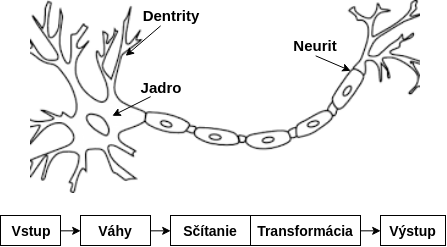
\includegraphics[width=0.5\linewidth]{img/bioneuron}
	\caption{Zjednodušený popis fungovania biologického neurónu}
	\label{fig:bioneuron}
\end{figure}

\indent Fungovanie biologického neurónu sa stalo inšpiráciou pre návrh umelého neurónu.
Rovnako ako biologický neurón, aj umelý neurón prijíma vstupné údaje - x\textsubscript{1},  x\textsubscript{2}, \dots,  x\textsubscript{n} ktoré sú násobené špecifickou váhou w\textsubscript{1},  w\textsubscript{2}, \dots,  w\textsubscript{n} prislúchajúcou k neurónu.
Váhované vstupy sú podobne ako pri biologickom neuróne sčítané, je k ním pripočítaný
základ(bias), a následne transformované aktivačnou funkciou, ktorej výsledok je odoslaný ďalším neurónom. Fungovanie neurónu sa dá zapísať ako rovnica\eqref{eqn:artneuron}, kde vstup, a jeho schému vidíme na obrázku\ref{fig:artneuron}.

\begin{figure}[H]
	\centering
	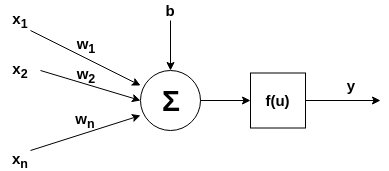
\includegraphics[width=0.7\linewidth]{img/artneuron}
	\caption{Schéma fungovania umelého neurónu}
	\label{fig:artneuron}
\end{figure}

\begin{equation}\label{eqn:artneuron}
y = f(\sum\limits_{i=1}^n x_{i}w_{i} + b)
\end{equation}

\indent Jedným neurónom vieme aproximovať jednoduchú lineárnu funkciu.
Na aproximáciu zložitejších problémov, napríklad na rozpoznanie ručne písaných znakov, ich však potrebujeme viac.
Ľudský mozog má usporiadané neuróny vo vrstvách.
Buduma tvrdí, že mozgová kôra, ktorá je zodpovedná za ľudské myslenie, je tvorená šiestimi takýmito vrstvami\cite{buduma2017fundamentals}, a informácia sa prenáša z jednej vrstvy do druhy, až kým vstupná informácia nedáva zmysel.
Príkladom je ľudské videnie, kde najspodnejšia vrstva prijíma informácie zo sietnice oka, táto informácia sa presúva vrstvami mozgovej kôry, až nakoniec v poslednej vrstve rozpozná, o aký predmet ide.\\

\indent Aplikovaním rovnakého konceptu spájania neurónov do vrstiev, vytvárame umelé neurónové siete.
Obrázok jednoduchej neurónovej siete vidíme na obrázku\ref{fig:ann}, kde spodná vrstva prijíma vstupné dáta a vrchná vrstva neurónov počíta finálny výsledok.
Stredná vrstva neurónov je nazývaná skrytá vrstva, kde $w_{i, j}^{(k)}$ označuje váhu prepojenia medzi í-tym v k-tej vrstve a j-tym neurónom v k+1 vrstve, pričom schopnosť neurónovej siete riešiť problémy 
priamo závisí na nájdení optimálnych hodnôt váh, pričom vďaka skrytej vrstve je možné vypočítať komplexnejšie vzťahy vo vstupných dátach.
V ukážkovej sieti sú existujú prepojenia neurónov v smere do nasledujúcej vrstvy, bez prepojení medzi neurónmi v rovnakej vrstve alebo do predchádzajúcej, tento typ siete sa označuje ako dopredná - feed forward.
Lineárne neuróny sú nenáročné na výpočet, avšak akákoľvek dopredná sieť len s lineárnymi neurónmi môže byť vyjadrená ako sieť bez skrytej vrstvy, a teda je limitovaná na naučenie sa zložitejších vzťahov.
Riešením je vnesenie nelineárnych vzťahov do neurónovej siete, prostredníctvom aktivačných funkcií.\cite{buduma2017fundamentals}

\begin{figure}[H]
	\centering
	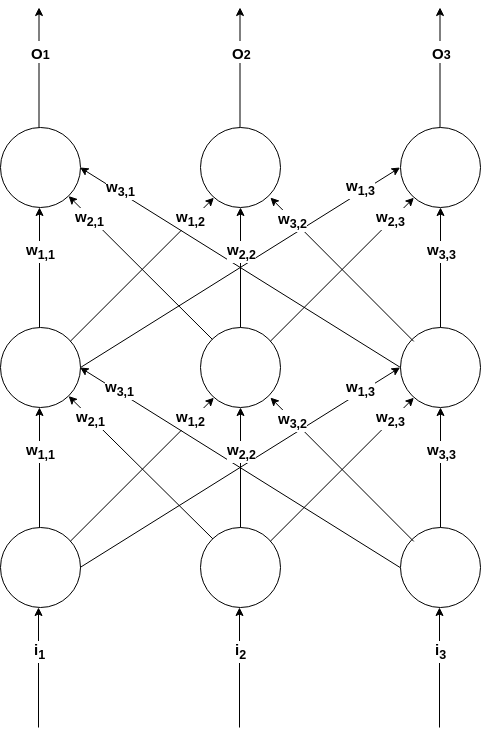
\includegraphics[width=0.5\linewidth]{img/ann}
	\caption{Príklad doprednej neurónovej vrstvy skladajúcej sa z troch vrstiev a tromi neurónmi vo vrstve.}
	\label{fig:ann}
\end{figure}

\subsection{Aktivačné funkcie}\label{activation}
Poznáme 3 základné nelineárne aktivačné funkcie - sigmoid, tanh a relu.
Sigmoidná funkcia, je definovaná ako\eqref{eqn:sigmoid}, jej priebeh na obrázku\ref{fig:sigmoid} je podobný písmenu s, čo spôsobuje, že ak je vstup veľmi malý, výstup bude blízky 0, a pokiaľ je veľmi veľký, výsledok sa blíži k 1.

\begin{equation}\label{eqn:sigmoid}
f(z) = \frac{1}{1 + e^{-z}}
\end{equation}

\begin{figure}[H]
	\centering
	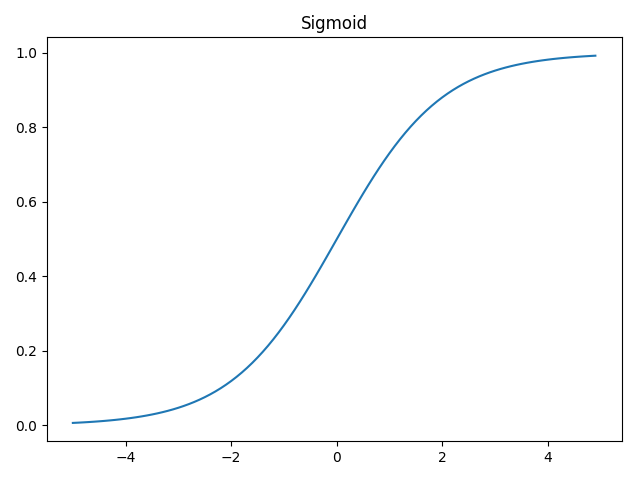
\includegraphics[width=0.5\linewidth]{img/sigmoid}
	\caption{Priebeh sigmoidnej funkcie}
	\label{fig:sigmoid}
\end{figure}

Funkcia tanh - hyperbolický tangens, je podobná sigmoidnej čo sa týka priebehu na obrázku\ref{fig:tanh}, s tým že jej rozsah je od -1 do 1, má centrum priebehu v 0, kvôli čomu je často preferovanou aktivačnou funkciou.

\begin{figure}[H]
	\centering
	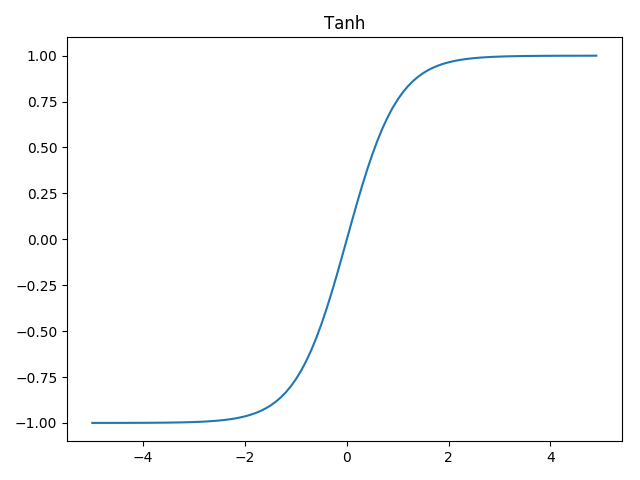
\includegraphics[width=0.5\linewidth]{img/tanh}
	\caption{Priebeh funkcie tanh}
	\label{fig:tanh}
\end{figure}

Iným tipom nelineárnej funkcie je Rectified Linear Unit(\acrshort{relu}), vyjadrený rovnicou \eqref{eqn:relu}, a priebehom ako na obrázku\ref{fig:relu} a je používanou funkciou najmä v oblasti strojového videnia.

\begin{equation}\label{eqn:relu}
f(z) = max(0, z)
\end{equation}

\begin{figure}[H]
	\centering
	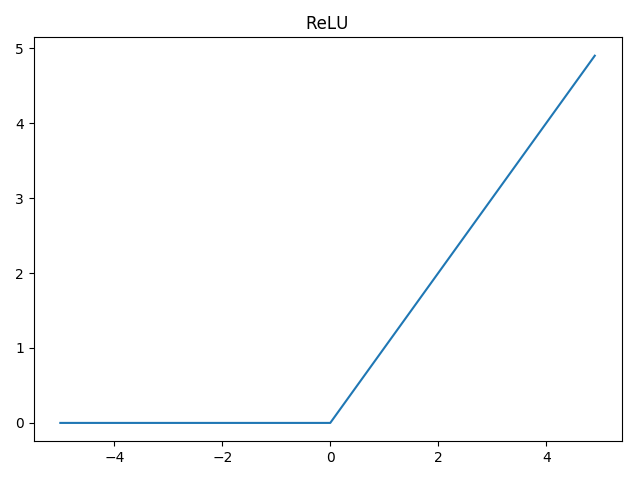
\includegraphics[width=0.5\linewidth]{img/relu}
	\caption{Priebeh ReLU funkcie}
	\label{fig:relu}
\end{figure}

\subsection{Trénovanie neuróvej siete}
Pod pojmom trénovania neurónovej siete rozumieme proces optimalizácie vektora váhových prepojení medzi neurónmi.
Počas trénovania sa zvyčajne na vstup neurónovej siete prináša veľké množstvo tréningových vzoriek, pričom opakovane upravujeme hodnoty váh s cieľom minimalizovať chybné výsledky neurónovej siete.
Chybu výsledku neurónovej siete vypočítame chybovou funkciou(objective function, error function loss function) \eqref{eqn:learning}, a kde $E$ je výsledná chyba pre i-tu tréningovú vzorku, $t^{i}$ označuje pravdivú hodnotu výsledku pre vzorku i a $y^{i}$ označuje výstup neurónovej siete.

\begin{equation}\label{eqn:learning}
E = \frac{1}{2} \sum \nolimits_{i} (t^{(i)} - y^{(i)})^2
\end{equation}

Výsledok chybovej funkcie je rovný nule, pokiaľ náš model neurónovej siete vracia perfektné výsledky pre každú trénovaciu vzorku.
Cieľom trénovania je teda optimalizovať váhy neurónov tak, aby sa výsledok chybovej funkcie E čo najviac približoval k E. 

\subsection{Gradient descent}\label{gd}
Po vypočítaní chybovej funckie je potrebné upraviť samotné hodnoty váh, pomocou metódy gradient descent.
Predpokladajme, že máme funkciu $y = f(x)$, kde obe $x$ a $y$ sú reálne čísla a derivácia tejto funkcie je označená
ako $f'(x)$.
Derivácia $f'(x)$ nám dáva sklon alebo smerovanie funcie $f(x)$ v bode $x$, inými slovami nám udáva, ako upraviť
malú zmenu vo vstupe tak, aby sme dosiahli požadovanú funkciu na výstupe\eqref{eqn:gd}. \cite{goodfellow2016deep}

\begin{equation}\label{eqn:gd}
f(x + e) \approx f(x) + ef'(x)
\end{equation}

\indent Derivácie sú vhodným prostriedkom na minimalizáciu funkcií, pretože nám udáva, ako upraviť x tak, aby sme dosiahli zlepšenie v y. 
Teda pokial vieme, že $f(x -  \epsilon (znamienko) (f'(x)))$ je menšie ako $f(x)$ pre malé $\epsilon$.
Môžeme teda zmenšiť $f(x)$ úpravou $x$ v malých krokoch v opačnom smere ako je $znamienko$ derivácie.
Táto technika sa nazýva gradient descent, a jej príklad vidíme na obrázku\ref{fig:gd}. \cite{goodfellow2016deep} \\

\begin{figure}[H]
	\centering
	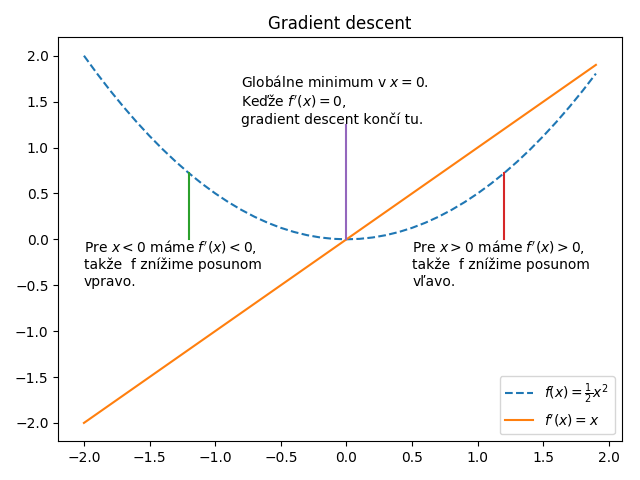
\includegraphics[width=1\linewidth]{img/gd}
	\caption{Ukážka, ako derivácie funkcie môže byť použitá na hľadanie minima funkcie (gradient descent)}
	\label{fig:gd}
\end{figure}

\indent V bodoch, kde $f'(x) = 0$, nemáme informáciu o tom, ktorým smerom sa má hodnota upraviť, a sú označované ako kritické alebo stacionárne body \cite{goodfellow2016deep}.
Lokálne minimum je bod, kde $f(x)$ je menšia ako všetky okolité body, takže nie je viac možné znížiť
hodnotu $f(x)$ vykonaním nekonečne malých krokov v jednom alebo druhom smere.
Analogicky lokálne maximum je body, kde $f(x)$ je väčšia ako všetky okolité body, takže nie je viac možné zvýšiť hodnotu $f(x)$ vykonaním nekonečne malých krokov v jednom alebo druhom smere.
Niektoré kritické body niesu ani minimom ani maximom a nazývajú sa sedlové body.\\

\indent Bod, kde $f(x)$ dosahuje absolútne najnižšiu hodnotu sa nazýva globálne minimum.
Je možné, aby mala funkcia jedno, alebo aj viac globálnych miním.
Tiež je možné, aby existovali lokálne minimá, ktoré niesu globálne optimálne.
V kontexte učenia neurónových sietí optimalizujeme funkcie, ktoré môžu mať veľké množstvo lokálnych miním, veľké množstvo sedlových bodov so širokými plochými oblasťami.
Toto všetko robí trénovanie neurónovej siete náročným, najmä pokiaľ ide o n-rozmerné dáta.
Kvôli tomu sa trénovanie siete často ukončí pri hodnote funkcie $f(x)$ ktorá je veľmi malá, ale 
nie nutne minimálne z formálneho hľadiska, ako vidíme na obrázku\ref{fig:gd_global_min}. \cite{goodfellow2016deep}

\begin{figure}[H]
	\centering
	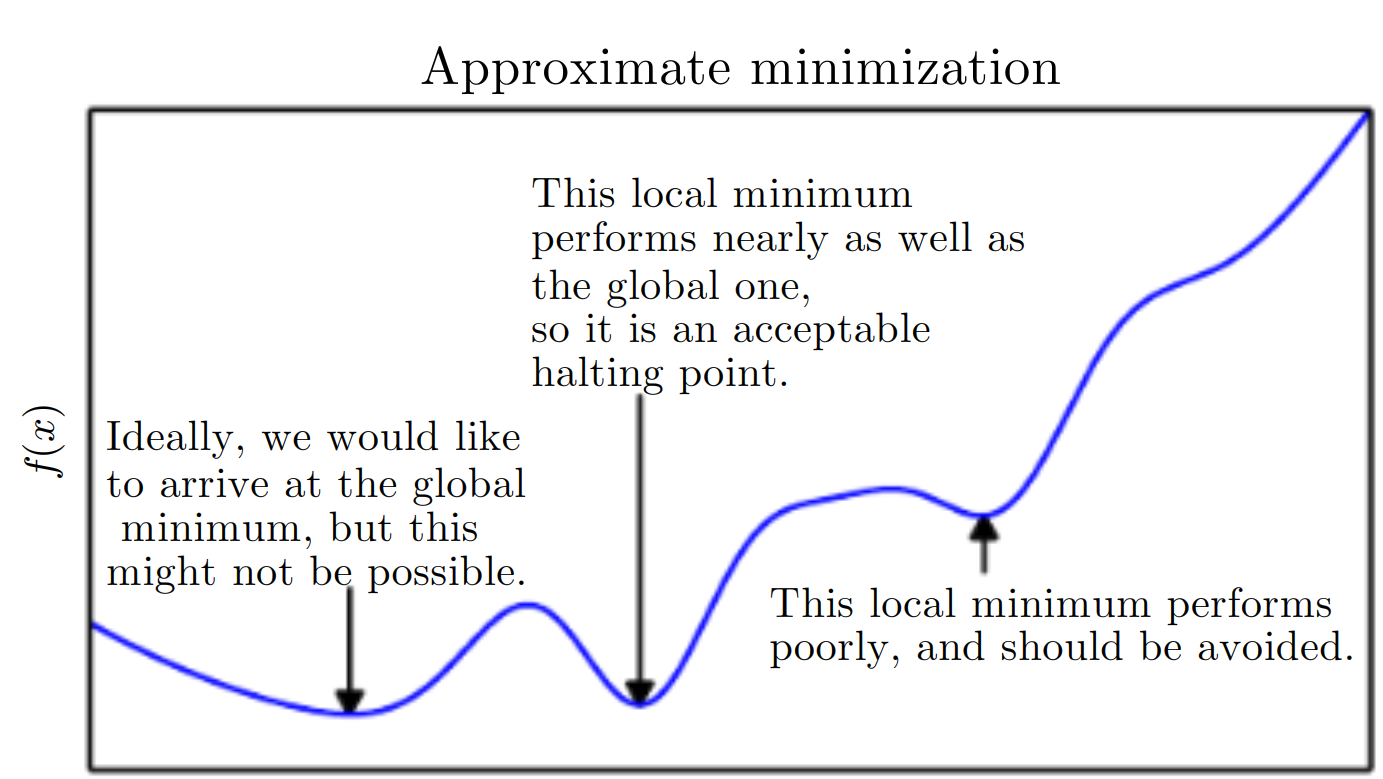
\includegraphics[width=0.75\linewidth]{img/gdglobalmin}
	\caption{Ukážka funkcie s niekoľkými lokálnymi minimami, prebraté z\cite[s.~85]{goodfellow2016deep}}
	\label{fig:gd_global_min}
\end{figure}

\subsection{Stochastic gradient descent} \label{l:sgt}
Stochastic gradient descent(\acrshort{sgd}) dôležitým a často používaným algoritmom pri učení neurónových sietí.
Ide o rozšírenie gradient descent algoritmu, ktorý sme popísali v\ref{gd}.\cite{goodfellow2016deep} \\

\indent Pri učení neurónových sietí sa snažíme dosiahnuť čo najlepšiu generalizáciu problému, k čomu je potrebné veľké množstvo trénovacích dát (dataset), ktoré sú však výpočtovo náročné.
Chybová funkcia používaná v strojovom učení je často založená na vypočítaní chyby pre každý prvok z trénovacích dát a ich následnom sčítaní, náročnosť tohoto výpočtu je $O(m)$ pre $m$ prvkov.
SGT tento problém rieši používaním menšieho počtu vzoriek (minibatch) pri výpočte chybovej funkcie, ktorých množstvo postačuje na určenie smeru optimalizácie chybovej funkcie. 
Použitie menšieho počtu vzoriek je kľúčovým aspektom pri trénovaní veľkých modelov neurónových sietí s veľkými trénovacími datasetmi.
Ak má model siete fixnú veľkosť, potom náročnosť SGD pri výpočte chyby v jednom cykle nezáleží od veľkosti trénovacieho datasetu $m$. \\

\indent Počet výpočtov chybovej funkcie pri klasickom gradient descent algoritme zvyčajne rastie v závislosti od počtru trénovacích prvkov.
S množstvom prvkov $m$ blížiacemu sa k nekonečnu, dosiahne model najlepší možný výsledok ešte predtým, než SGD použije všetky prvky trénovacieho datasetu.
Zvyšovaním množstva prvkov v datasete v takomto prípade už nenavýši množstvo času potrebného na dosiahnutie najlepšieho možného výsledku.
Z tohoto uhla pohľadu je možné tvrdiť, že približná náročnosť trénovania modelu pomocou SGD sa rovná $O(1)$, ako funkcií $m$.\cite{goodfellow2016deep}

\subsection{Generalizácia, overfitting a underfitting}
Hlavným cieľom strojového učenia aby model fungoval dobre nielen na trénovacích dátach, ale najmä 
na úplne nových vstupných dátach.
Schopnosť neurónovej siete správne fungovať aj na nových dátach nazývame generalizácia. \\

\indent Pri trénovaní neurónovej siete sa využíva trénovací dataset, na ktorom sa počíta trénovacia chyba, ktorú sa snažíme minimalizovať.
Tento proces môžeme zaradiť zaradiť medzi jednoduché optimalizačné problémy.
Čo však oddeľuje strojové učenie od optimalizácie je snaha dosiahnuť aj nízku generalizačnú chybu, tiež označovanej ako testovacia chyba a je  definovaná ako hodnota chyby na nových dátach.\cite{goodfellow2016deep}. \\

\indent Testovaciu chybu modelu neurónovej siete získavame meraním úspešnosti na testovacom datasete, pričom vzorky z testovacieho datasetu sa nenachádzajú v trénovacom datasete - teda sú úplne nezávislé, rozdelené rovnomerným spôsobom.
Pri výpočte testovacej chyby chyby sa do neurónovej siete privedú vzorky z trénovacieho datasetu, vypočíta sa trénovacia chyba, optimalizujú sa parametre - váhy tak aby sa znížila trénovacia chyba - tento proces sme popísali v kapitole\ref{gd}, potom sa na vstup neurónovej siete privedú vzorky z testovacieho datasetu a vypočíta sa testovacia chyba, ktorá je väčšia alebo rovná trénovacej chybe\cite{goodfellow2016deep}.

Faktory, ktoré určujúc úspešnosť neurónovej siete, sú schopnosti:

\begin{itemize}
	\item Minimalizovať trénovaciu chyby
	\item Udržať čo najmenšiu vzdialenosť medzi testovacou a trénovacou chybou
\end{itemize}
\cite{goodfellow2016deep}

\indent Tieto dva faktory faktory korešpondujú dvom problémom strojového učenia - nedotrénovanie (underfit) a pretrénovanie(overfit).
Undefitting znamená, že model siete nie je schopný dosiahnuť požadovanú hodnotu chyby na trénovacom datasete.
Pretrénovanie označuje situáciu, kedy je rozdiel medzi trénovacou a testovacou chybou príliš veľký.
Kapacitou modelu (capacity), je možné kontrolovať, či bude sieť náchylnejšia k nedotrénovaniu alebo pretrénovaniu.
Kapacitou modelu myslíme schopnosť modelu obsiahnuť širokú škálu funkcií\cite{goodfellow2016deep}.
Modely s nižšou kapacitou môžu mať problém pri naučení sa zložitejších funkcií trénovacích dát,
zatiaľ čo modely s vyššou kapacitou sú náchylné k naučeniu sa takých vlastností trénovacieho datasetu, ktoré zvyšujú chybovosť testovacieho datasetu.
Vo všeobecnosti teda platí, že model funguje najlepšie v prípade, ak kapacita modelu korešponduje so skutočnou komplexitou problému, ktorý sa sieť model snaží naučiť \cite{lawrence1997lessons}. \\

\indent Na obrázku\ref{fig:capacity} vidíme názornú ukážku týchto princípov, na ktorom porovnávame model s kapacitou na predikovanie lineárnych, kvadratických a 9 dimenzionálnych funkcií, pričom skutočným cieľom je predikovanie kvadratických funkcií. Linerána kapacita nie je schopná poňať celú podstatu kvadratickej funkcie, a preto je model podtrénovaný. Model o kapacite 9 je schopný poňať kvadratickú funkciu, avšak jeho rozsah dovoľuje natrénovať nekonečné množstvo iných funkcií so správnymi hodnotami pre trénovacie dáta, pretože má model viac parametrov než máme trénovacích dát. 

\begin{figure}[H]
	\centering
	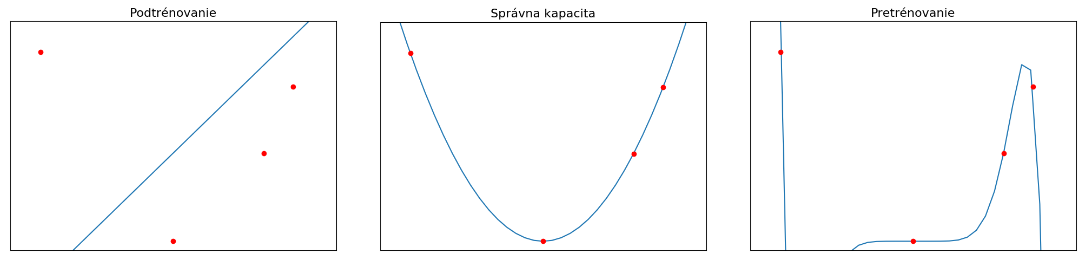
\includegraphics[width=1\linewidth]{img/capacity}
	\caption{Kapacita siete a jej vzťah k nedotrénovaniu a pretrénovaniu}
	\label{fig:capacity}
\end{figure}

\indent Ukážku trénovacej a testovacej chyby a ich vzťahu s podtrénovaním a pretrénovaním vidíme na obrázku\ref{fig:errors}.

\begin{figure}[H]
	\centering
	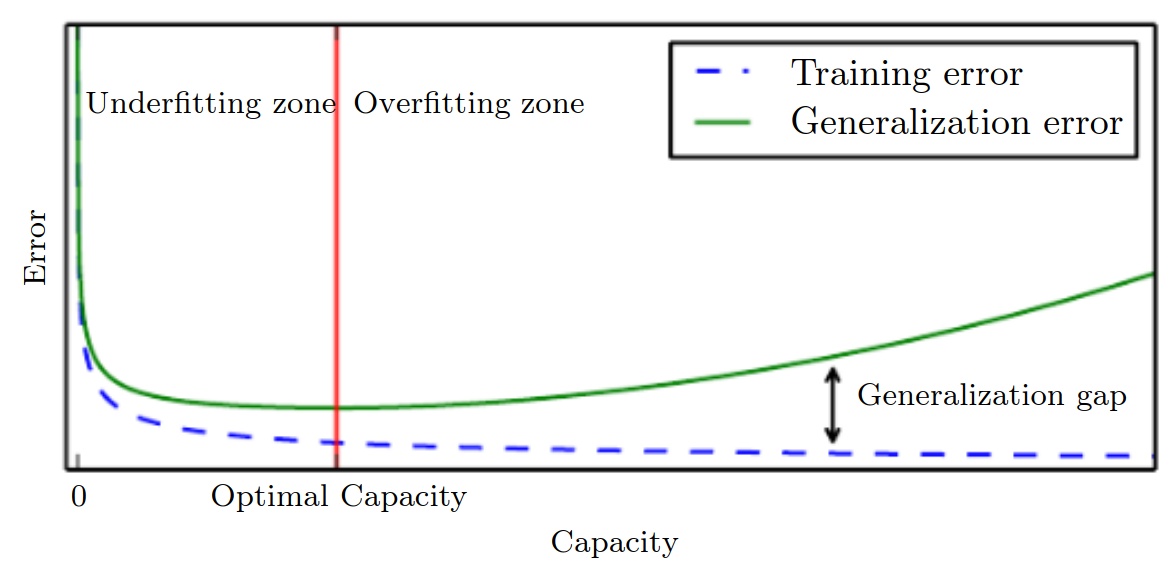
\includegraphics[width=.5\linewidth]{img/errors}
	\caption{Vzťah medzi kapacitou a chybou trénovania,  prebratá z z\cite[s.~115]{goodfellow2016deep}}
	\label{fig:errors}
\end{figure}

\subsection{Regularizácia}
Ako sme už spomenuli, hlavným cieľom pri strojovom učení je vytvoriť taký model, ktorý bude fungovať správne nielen na trénovacích dátach, ale taktiež na nových neznámych vzorkách.
Veľké množstvo algoritmov strojového učenia je špeciálne navrhnutých tak, aby minimalizovali testovaciu chybu, hoci za cenu vyššej trénovacej chyby.
Tieto prístupy pri učení neurónových sietí označujeme ako regularizácia\cite{nielsen2015chapter}.
Najčastejšie ide o pridanie nových pravidiel do modelu neurónovej siete, ako napríklad obmedznie možných hodnôt parametrov neurónovej siete či pridanie pravidiel do chybovej funkcie, čo môžeme tiež chápať ako nepriame obmedzenie hodnôt parametrov v neurónovej sieti \cite{goodfellow2016deep}.
Za predpokladu, že sú tieto pravidlá a obmedzenia vybrané vhodne, môžu viesť k lepším výsledkom na testovacom datasete.

\subsubsection{$L^2$ regularizácia}
$L^2$, tiež známa ako úpadok váh(weight decay), je regularizáciou, ktorá približuje váhy smerom k pôvodnej hodnote - najčastejšie k 0 tým, že do chybovej funkcie zavádza vzťah \eqref{eqn:l2} \cite{Regulari14}.

Tento vzťah vyjadruje, že $L^2$ spôsobuje, že stupné dáta si zachovávajú vyššiu varianciu,  čím znižuje hodnoty váh príznakov, ktorých kovariancia na cieľovom výstupe je nízka v porovnaní s varianciou vstupu. \cite{van2017l2}.

\begin{equation}\label{eqn:l2}
	L^2 = \frac{1}{2} \parallel w \parallel^2_{2} = \frac{1}{2}\sum\limits_{i=0}^n w^2_{i}
\end{equation}

\indent Tento vzťah môžeme tiež chápať tak, že váhy ktorých hodnota je blízka nule majú nízky vplyv na komplexitu modelu, zatiaľ čo vzdialenejšie hodnoty majú obrovský vplyv \cite{Regulari14}.

\subsubsection{$L^1$ regularizácia}
$L^2$ regularizácia je pravdepodobne najpoužívanejšia pri redukovaní hodnôt váh, okrem nej však existujú aj iné druhy regularizácií ktoré zmenšujú veľkosť modelu - napríklad $L^1$, ktorá je definovaná vzťahom \eqref{eqn:l1} \cite{goodfellow2016deep}.
\begin{equation}\label{eqn:l1}
	L^1 =  \parallel w \parallel{+} = \sum\limits_{i=0}^n \lvert w_{i} \rvert_{i}
\end{equation}

\indent V porovnaní s $L^2$ je výsledkom $L^1$ regularizácie redší model, čo znamená, že väčšie množstvo parametrov môže dosiahnuť presnú hodnotu 0, na rozdiel od $L^2$, kde sa hodnota parametrov len približuje k 0.\cite{Regulari75}. 
Toto môžeme chápať ako mechanizmus selekcie použitých príznakov, čím sa zjednodušuje proces učenia neurónovej siete, keďže sa zníži množstvo parametrov, ktoré sa použijú.

\subsection{Konvolučné neurónové siete}
Konvolučné neurónové siete sú špeciálnym druhom neurónových sietí ktoré majú topológiu podobnú mriežke, ako napríklad time-series dát, reprezentovateľné ako 1-rozmerná mriežka, alebo obrázkové dáta, v ktorých sú pixely usporiadané ako 2-rozmerná mriežka\cite{goodfellow2016deep}.

Vrstvy konvolučnej neurónovej siete sa v bežnom prípade skladajú z troch základných krokov, ako vidíme aj na obrázku\ref{fig:convo}, v literatúra sa často uvádzajú tiež ako osobitné vrstvy:
\begin{itemize}
	\item Konvolúcia
	\item Detekcia (ReLU)
	\item Pooling
\end{itemize}


\begin{figure}[H]
	\centering
	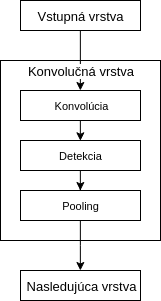
\includegraphics[width=0.2\linewidth]{img/convo}
	\caption{Diagram vrstvy konvolučnej neurónovej siete}
	\label{fig:convo}
\end{figure}


\subsubsection{Konvolúcia}
Názov konvolučná neurónová sieť je založený na matematickej operácii - konvolúcii. 
Tá je založená na troch základných bodoch, ktoré zlepšujú učenie neurónovej siete:
\begin{itemize}
	\item Redšie prepojenia (sparse interactions)
	\item Zdieľanie parametrov (parameter sharing)
	\item Ekvivariantné vyjadrenia (equivariant representations)
\end{itemize}
\cite{goodfellow2016deep}.\\

\indent Tradičné vrstvy neurónové siete sú postavené na násobení matice parametrov s maticou parametrov (váhami), medzi každým vstupným a každým výstupným neurónom - čo znamená, že každý neurón vstupnej vrstvy ovplyvňuje všetky neuróny výstupnej vrstvy.
Konvolučné neuróné siete sa v tomto odlišujú, pretože používajú redšie prepojenia, čo je dosiahnuté použitím menšieho jadra než je vstup(kernel).
Napríklad, pri spracovaní obrázkových dát, ktoré pozostávajú z miliónov pixelov, detekujeme menšie príznaky ako napríklad hrany, v podoblasti len niekoľkých stoviek pixelov. \cite{goodfellow2016deep}
Teda, pokiaľ máme $m$ vstupných neurónov a $n$ výstupných, potom maticové násobenie vyžaduje $m \times n$ parametrov, a teda náročnosť takejto operácie je $O(m \times n)$.
Ak však zmenšíme množstvo prepojení na $k$, potom je potrebných $k \times n$, s náročnosťou $O(k \times n)$, pričom v praxi je možné dosiahnuť dobré výsledky trénovania pri použití $k$, ktoré je omnoho menšie ako $m$.
To znamená, že je potrebný menší počet parametrov, čo šetrí pamäťové prostriedky, znižuje množstvo operácií, ktoré je potrebné vykonať, a vo všeobecnosti výrazným spôsobom zlepšuje efektivitu trénovania modelu.
Názornú demonštráciu redších prepojení vidíme na obrázku\ref{fig:sparse} a ukážku plný prepojení na obrázku\ref{fig:fully}. 
 
\begin{figure}[H]
	\centering
	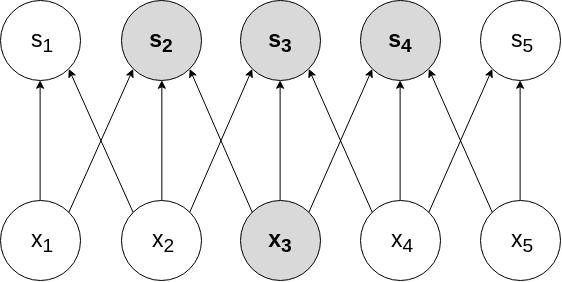
\includegraphics[width=0.5\linewidth]{img/sparse}
	\caption{Ukážka redšieho prepojenia neurónov so zvýraznením prepojení, ktoré má neurón $x_{3}$ }
	\label{fig:sparse}
\end{figure}

\begin{figure}[H]
	\centering
	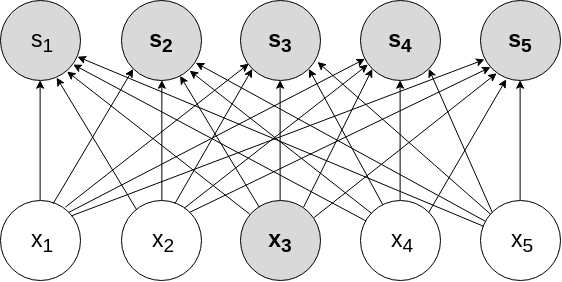
\includegraphics[width=0.5\linewidth]{img/fully}
	\caption{Ukážka plných prepojení neurónov so zvýraznením prepojení, ktoré má neurón $x_{3}$} 
	\label{fig:fully}
\end{figure}

\indent Zdieľanie parametrov znamená, že rovnaké parametre sú použité vo viacerých funkciách modelu.
Pri klasických neurónových sieťach je každý element matice váh použitý práve jeden krát, s jedným  elementom zo vstupu, pri výpočte výstupu pre nasledujúcu vrstvu.
Pri konvolučných neurónových sieťach sa každý prvok jadra použije spolu s každým elementom zo vstupu(okrem hraničných v závislosti od návrhu modelu - padding, stride \dots). Zdieľanie parametrov teda znamená, že namiesto učenia osobitných skupín parametrov pre každú pozíciu zo vstupu, sa sieť naučí len jednu, ktorá je použítá pre všetky lokácie.\cite{goodfellow2016deep} \\

\indent Vďaka zdieľaniu parametrov nadobúdajú vrstvy neurónovej siete vlastnosť ekvivariancie voči presunom.
Funkcia je ekvivariantná, pokiaľ zmeny vstupu ovplyvňujú zmeny vo výstupe rovnakou mierou, a teda, 
funkcia $f(x)$ je ekvivariantná k funkcii $g$, ak $g(f(x)) = f(g(x))$.
V prípade konvolúcie, nech $g$ je funkcia ktorá, sa presúva po vstupe, je funkcia $g$ ekvivariantná funkcií konvolúcie.
Táto vlastnosť je obzvlášť výhodná, pokiaľ chceme na celom vstupe detegovať rovnaké príznaky - napríklad hrany, naopak nemusí pokiaľ chceme v rôznych častiach obrázka detegovať iné príznaky - napríklad vo vrchnej časti obrázka detegovať obočie, a v spodnej bradu. \cite{goodfellow2016deep} \\

\indent Na obrázku\ref{fig:cnn1} vidíme jednoduchý príklad operácie konvolúcie, kde tmavomodrá mriežka  predstavuje vstupnú mapu príznakov(input feature map).
Pre zjednodušenie použijeme príklad len s jednou mapou príznakov, avšak v bežnej praxi ich môže byť niekoľko naskladaných jedna na druhej.
Šedá oblasť ktorá sa označuje ako jadro, posúvame naprieč mapou príznakov.
Pre každú podoblasť mapy príznakov je vypočítaný výstup vychádzajúci z danej podloblasti, ktorých sčítanie tvorí výstup danej podoblasti.\cite{dumoulin2016guide}
Tento postup môže byť zopakovaný $n-krát$ použitím rôznych jadier, čím vznikne $n$ výstupných máp príznakov, výstupná mapa príznakov je označená zelenou farbou.
Pokiaľ máme niekoľko vstupných máp vstupujúcich do konvolúcie, potom je potrebné použiť 3-rozmerné jadro, alebo, každá zo vstupných máp použije odlišné jadro, ktorých výsledok bude následne sčítaný do výstupnej mapy príznakov.\\
\indent Príklad na obrázku\ref{fig:cnn1} zobrazuje 2-rozmernú konvolúciu, avšak môže byť  použitý na generalizovanie aj n-rozmernej konvolúcie.
V prípade 3-rozmernej konvolúcie by jadro predstavovalo kváder, ktorým by sme prechádzali naprieč výškou, šírkou a hĺbkou vstupnej mapy príznakov.\cite{dumoulin2016guide} \\

\indent Súbor jadier predstavujúcich konvolúcie má tvar korešpondujúci permutácii $(n, m, k_{1}, \dots, k_{N})$ kde $n$ označuje počet výstupných máp príznakov, $m$ označuje počet vstupných máp príznakov a $k_{j}$ označuje veľkosť jadra pozdĺž osi $j$.\cite{dumoulin2016guide}

 
\begin{figure}[H]
	\centering
	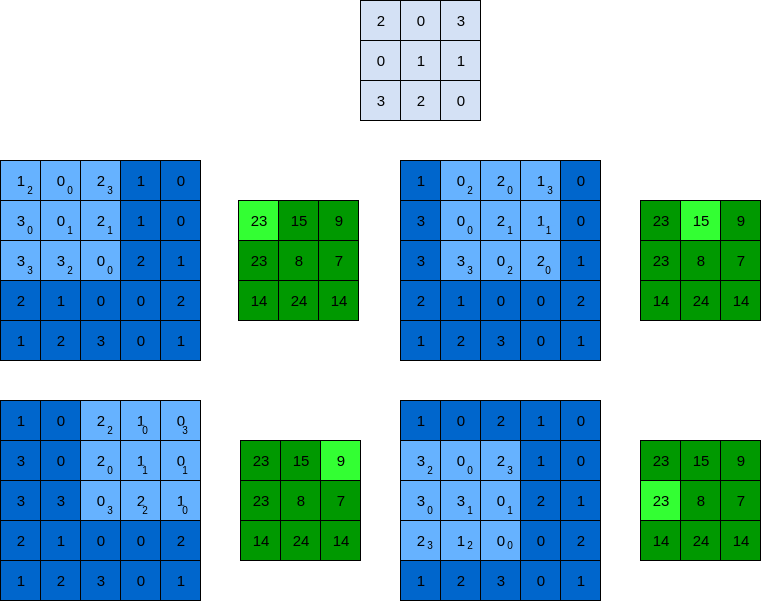
\includegraphics[width=1\linewidth]{img/cnn1}
	\caption{Výpočet výstupných hodnôt operácie konvolúcie}
	\label{fig:cnn1}
\end{figure}

\indent Výstupnú veľkosť $o_{j}$ konvolučnej vrstvy pozdĺž osi $j$ ovplyvňuje niekoľko parametrov:

\begin{itemize}
	\item $i_{j}$: vstupná veľkosť(input size) pozdĺž osi j
	\item $k_{j}$: veľkosť jadra(kernel size) pozdĺž osi j
	\item $s_{j}$: vzdialenosť medzi dvomi po sebe nasledujúcimi podoblasťami(stride) pozdĺž osi j
	\item $p_{j}$: veľkosť okraja(padding) pozdĺž osi j
\end{itemize}

\indent Na obrázku\ref{fig:cnn2} ukazuje použitie jadra  o veľkosti $3 \times 3$, použitého na vstupe o veľkosti $5 \times 5$, okrajom $1 \times 1$ s hodnotami $0$ a stridom $2 \times 2$.

\begin{figure}[H]
	\centering
	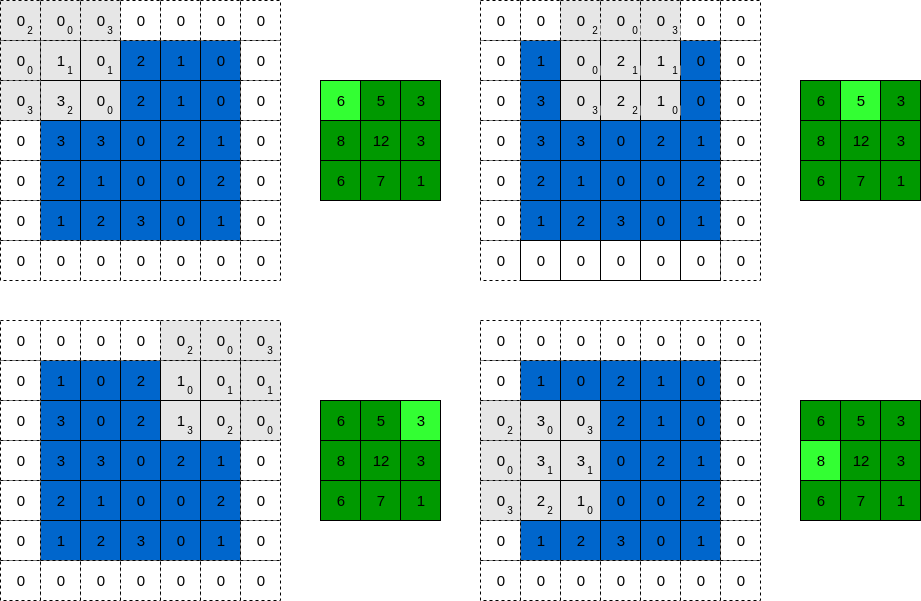
\includegraphics[width=1\linewidth]{img/cnn2}
	\caption{Výpočet výstupných hodnôt konvolúcie s použitím paddingu a stridu }
	\label{fig:cnn2}
\end{figure}

\subsubsection{Pooling}
Vo fáze detekcie prejde výstup konvolúcie aktivačnou funkciou ReLU, ktorú sme spomenuli v časti\ref{activation}. Výstup z fázy detekcie pokračuje do funkcie poolingu, ktorá ďalej upraví výstup do ďalšej vrstvy.\\ 

\indent Ide o aplikáciu poolingovej funkcie na vstupné dáta, čím dôjde k zmenšeniu výsledku.
Podobne ako pri konvolúcií, prechádzame vstup krok po kroku, avšak namiesto lineárnej operácie používanej pri konvolúcii, použijeme štatistickú funkciu, hľadajúci napríklad maximálne, priemerné či minimálne hodnoty v danej oblasti \cite{cs231n}.
Vo všetkých týchto prípadoch, napomáha pooling vytvoriť výstup, ktorý je invariantný voči malým zmenám pozičným posunom vstupu - to znamená, že pokiaľ sa sa vstup do funkcie poolingu zmení len o malú hodnotu, potom sa väčšina dát vo výstupe poolingu nezmení. 
Invariancia voči malým lokálnym zmenám môže byť veľmi užitočná, pokiaľ je väčším cieľom detegovať, či sú príznaky vôbec prítomné, než detegovať kde presne sú\cite{goodfellow2016deep}.
Napríklad, ak je naším cieľom detegovať, či obrázok obsahuje tvár, potom nepotrebujeme zisťovať presnú polohu očí na pixel presne, stačí, že vieme zistiť, že tvár má oči na oboch stranách. \\

\indent Poolingová funkcia použitá na riedke oblasti vytvára invarianciu voči posunom, avšak ak použijeme pooling na nezávislé parametrizované konvolúcie, potom je možné, že sa príznaky samé naučie, voči ktorým príznakom sa majú stať invariantnými\cite{goodfellow2016deep}. \\

\indent Pretože pooling sumarizuje výsledok z celej oblasti, potrebujeme menšie množstvo jednotiek vykonávajúcich pooling než jednotiek detektora, vďaka tomu, že bedú do úvahy oblasti o veľkosti $k$ pixelov, namiesto 1 pixelu, ako vidíme aj na obrázku\ref{fig:pooling}.
Tým sa zvyšuje výpočtová efektivita vrstvy neurónovej siete, pretože ďalšia vrstva má $k$ krát menší vstup, ktorý potrebuje spracovať.\cite{goodfellow2016deep} \\

\begin{figure}[H]
	\centering
	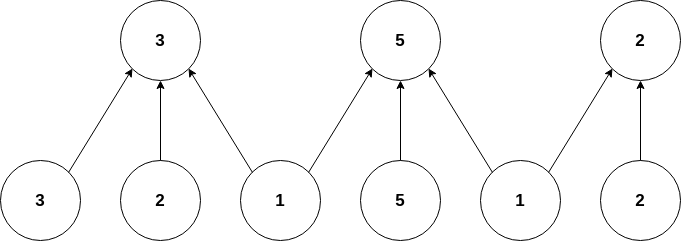
\includegraphics[width=0.5\linewidth]{img/pooling}
	\caption{Max pooling spolu s downsamplingom z pohľadu prepojení neurónov}
	\label{fig:pooling}
\end{figure}

Veľkosť výstupu $o_{j}$ a fungovanie poolingu ovplyvňuje niekoľko parametrov.

\begin{itemize}
		\item $i_{j}$: vstupná veľkosť(input size) pozdĺž osi j
		\item $k_{j}$: veľkosť polingovej podoblasťami(pooling window) pozdĺž osi j
		\item $s_{j}$: vzdialenosť medzi dvomi po sebe nasledujúcimi podoblasťami(stride) pozdĺž osi j
\end{itemize}

Príklad ich použitia vidíme na obrázku\ref{fig:poolingex}, kde $i = 5 \times 5$, $k = 3 \times 3$ a  $s = 1 \times 1$:

\begin{figure}[H]
	\centering
	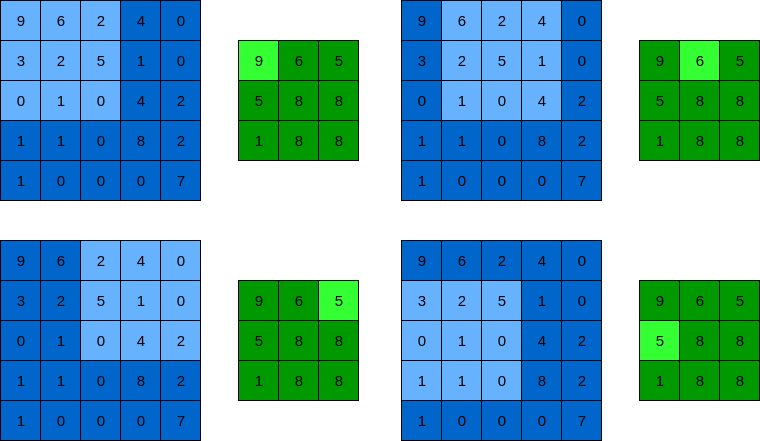
\includegraphics[width=1\linewidth]{img/poolingex}
	\caption{Výpočet výstupných hodnôt použitím max poolingu}
	\label{fig:poolingex}
\end{figure}

\newpage 

\section{Model neurónovej siete na rozpoznávanie tvárí}\label{l:fcnt}
Cieľom tejto práce je aplikovať natrénovaný model konvolučnej neurónovej siete pri rozpoznávaní tváre na zariadení Android OS.
Tento cieľ je teda možné rozdeliť na dve základné časti:
\begin{enumerate}
	\item Natrénovanie modelu neurónovej siete
	\item Aplikácia modelu na zariadení Android OS.
\end{enumerate}

Táto kapitola sa bude venovať prvému budu - vytvoreniu natrénovaného modelu neurónovej siete.
V našom prípade sme netrénovali celú sieť na rozpoznávanie tváre, ale použili sme model neurónovej siete Facenet, ktorá je schopná extrahovať príznaky tváre, 
ktoré budú použité pri klasifikácii.

\subsection{Facenet}
Pri popise tohoto modelu neurónovej siete sa budeme opierať najmä o článok \cite{schroff2015facenet},
v ktorom je detailne popísaná štruktúra Facenetu a problémov ktoré rieši.
Taktiež využijeme poznatky Sandberga, ktorý vytvoril voľne dostupnú implementáciu Facenetu na \url{https://github.com/davidsandberg/facenet}, a ktorá sa v súčastnosti ďalej vyvíja.
Chceme upozorniť, že v tejto práci sme vychádzali a upravovali implementáciu Facenetu z konca roka 2017, vhľadom k tomu, že v súčastnosti sa jeho implementácia pozmenila.\\
 
\indent Ide o model neurónovej siete, navrhnutý na rozpoznávanie tvárí pre rôzne možnsti aplikácie - identifikácie, verifikácie či clusteringu(hľadanie a spájanie rovnakých tvári).
Je založený na učení sa príznakov v Euklidovskom priestore (Euclidean embedding) obrázkov prostredníctvom hlbokej konvolučnej siete.
Sieť je trénovaná tak, aby umocnené $ L^2 $ vzdialenosti v podpriestore príznakov priamo poukazovali na podobnosť tvárí - teda podobné tváre majú nižšiu vzdialenosť než odlišné tváre \cite{schroff2015facenet}.
Po vypočítaní príznakov tváre je ďalší krok rovnaký ako pri iných klasifikačných problémoch - vypočítanie vzdialenosti medzi príznakmi dvoch tvári a určeniu či ide o rovnaké tváre na základe thresholdu v prípade verifikácie alebo k-NN(k nearest neighbors) klasifikačný problém v prípade identifikácie.\\

\indent Facenet sa odlišuje od ostatných prístupov k rozpoznávaniu tvárí pomocou hlbokých neurónových sietí, menovite článok \cite{schroff2015facenet} porovnáva prístup voči \cite{wst2008deeply}, kde bola použitá stredná vrstva neurónovej siete natrénovanej na známych inentitách, na všeobecné rozpoznávanie tvárí mimo trénovacieho datasetu.
``Nevýhodou tohoto prístupu je však nepriamosť a neefektivita: je nutné dúfať, že reprezentácie tváre strednou vrstvou je dostatočne generalizovaná voči novým tváram; použitím strednej vrstvy na vznikajú veľké(1000 - rozmerné) reprezentácie tvárí``\cite{schroff2015facenet}. 
Túto dimenzionalitu je možné síce redukovať pomocou PCA podobne ako v \cite{wst2008deeply}, avšak ide len o lineárnu transformáciu príznakov, čím nemusíme nutne zaručiť dostatočnú generalizáciu na nové tváre. \\

\indent Prístup Facenetu je odlišný v tom, že priamo trénuje neurónovú sieť do 128-rozmerného výstupu, pričom trénovanie je založené chybovej funkcií využívajúcej trojice založenej na LMNN(Large margin nearest neighbor)\cite{weinberger2009distance}.
Chybová funkcia Facenetu teda pracuje s trojicami, ktoré pozostavajú z dvoch tvárí rovnakej identity a jednej odlišnej, čím dosahuje väčšiu vzdialenosť v priestore medzi tvárami odlišných identít a naopak nižšiu medzi tvárami rovnakej identity.
Na trénovanie využíva orezané obrázky tvárí, na ktoré nebolo aplikované žiadne špeciálne 2-rozmeré alebo 3-rozmerné zarovnanie, okrem škálovania a posunu. \\

\indent Zjednodušený diagram fungovania Facenetu vidíme na obrázku\ref{fig:facenet}

\begin{figure}[H]
	\centering
	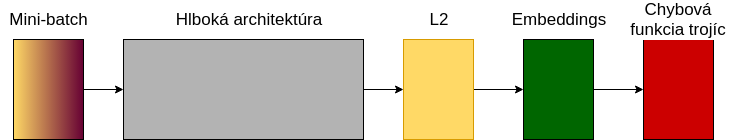
\includegraphics[width=1\linewidth]{img/facenet}
	\caption{Diagram fungovania Facenetu}
	\label{fig:facenet}
\end{figure}

\subsubsection{Chybová funkcia}
Prostredníctvom chybovej funkcie trojíc sa sieť usiluje o zapuzdrenie $f(x)$, vstupného obrázka $x$ do $d$-rozmerného Euklidovského priestoru príznakov $R^d$, $f(x) \in R^d$, aby umocnená vzialenosť medzi všetkými tvárami, nezávisle na variácií póz, osvetlenia či iných podmienok, medzi rovnakými tvárami bola nízka, zatiaľ čo vzdialenosť medzi obrázkami tvárí rozdielnych bola veľká, obrázok\ref{fig:triplet}\cite{schroff2015facenet}.
Okrem toho zavádza ďalšie pravidlo $\parallel f(x) \parallel_{2} = 1$ čím omedzuje vnorenie na 
$d$-rozmernú hyperguľu.

\begin{figure}[H]
	\centering
	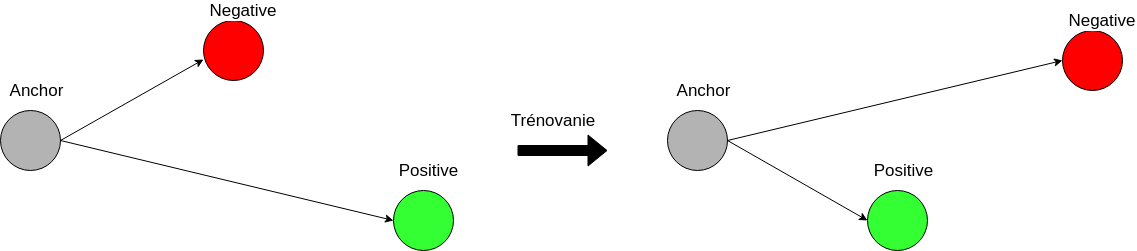
\includegraphics[width=0.75\linewidth]{img/triplet}
	\caption{Ukážka princípu úpravy vzdialeností medzi vzorkami pri chybovej funkcii trojíc}
	\label{fig:triplet}
\end{figure}

Túto chybovú funkciu vieme vyjadriť ako rovnicu \eqref{eqn:tripletl} \eqref{eqn:tripletl2}, kde $x_{i}^a$ označuje vstupnú vzorku(anchor), $x_{i}^p$ označuje zhodnú identitu(positive), ktorú chceme priblížiť vstupu,
$x_{i}^n$ inú osobu(negative), $\alpha$ vyjadruje vynútený rozostup medzi pozitívnym a negatívnym párom a $\tau$ označuje všetky možné trojice obrázkov s kardinalitou $ N $ \cite{schroff2015facenet}.

\begin{equation}\label{eqn:tripletl}
\parallel f(x_{i}^a) - f(x_{i}^p) \parallel_{2}^2 + \alpha <
\parallel f(x_{i}^a) - f(x_{i}^n)\parallel_{2}^2
\end{equation}

\begin{equation}\label{eqn:tripletl2}
\forall(f(x_{i}^a), f(x_{i}^p), f(x_{i}^n)) \in \tau
\end{equation}

\indent Výsledná chybová funkcia má potom tvar \eqref{eqn:tripletlf} \cite{schroff2015facenet}.

\begin{equation}\label{eqn:tripletlf}
\sum \limits_{i}^N [
\parallel f(x_{i}^a) - f(x_{i}^p) \parallel_{2}^2 -
\parallel f(x_{i}^a) - f(x_{i}^n) \parallel_{2}^2 + \alpha 
]_{+}
\end{equation} 

\subsubsection{Výber trojíc}
Vhodný výber trojíc sa ukázal ako kľúčový pre rýchlu konvergenciu k dobrým výsledkom, a teda
vybrať také trojice, aby porušovali rovnicu \eqref{eqn:tripletl}, čo znamená, že pre zvolený vstup
$x_{i}^a$ chceme vybrať také $x_{i}^p$, aby sme dosiahli $argmax_{x_{i}^p}\parallel f(x_{i}^a) - f(x_{i}^p) \parallel_{2}^2$ a podobne $x_{i}^n$ také aby spĺňalo $argmin_{x_{i}^n}\parallel f(x_{i}^a) - f(x_{i}^n) \parallel_{2}^2$. 

Autori článku\cite{schroff2015facenet} o Facenete udávajú, že je nemožné počítať $ argmin $ a $ argmax $ cez celý tréningový dataset kvôli výpočtovej náročnosti, a navrhujú dve možné riešenia výberu trojíc:

\begin{itemize}
	\item Generovať trojice offline každých n krokov a počítať $ argmin $ a $ argmax $ na podmnožine dát
	\item Generovať trojice online, výberom pozitívnej a negatívnej vzorky z mini-batchu(dávky v jednom cykle) 
\end{itemize}

\indent Z týchto dvoch možností autori zvolili možnosť online generovania s použitím väčších - niekoľko-tisícových mini-batchov, v ktorých sa nachádza približne 40 vzoriek pre jednu identitu. \\

\indent Model bol trénovaný pomocou SGD algoritmu, ktorý sme popísali v\ref{l:sgt}.
Autori testovali 4 rôzne architektúry typu Inception, líšiacich sa vo veľkosti vstupu(220x220 - 96x96) či hĺbke siete a množstve potrebnej výpočtovej sily(220 mil. FLOPS - 20 mil. FLOPS), a ich porovnanie výsledkov vidíme na obrázku\ref{fig:facenetflops}, a dosiahli úspešnosť na LFW datasete $ 99,63\% +- 0.09 $ s použitím zarovnani tvárí.
Z výsledkoch ich pokusov je tiež zaujimavé, že dimenzionalita príznakov na ktoré trénovali neurónové siete je prekvapivo najvhodnejšia pri 128 rozmeroch, kde dosiahli najlepšie výsledky v porovnaní so 64, 256 a 512 dimenzií.
Tieto výsledky dosiahli na veľkosti snímkov o rozmeroch $ 220 \times 220 $, avšak poukázali na to, že menšie snímky o veľkosti $ 120 \times 120 $ dosahujú len o málo horšie výsledky.

\begin{figure}[H]
	\centering
	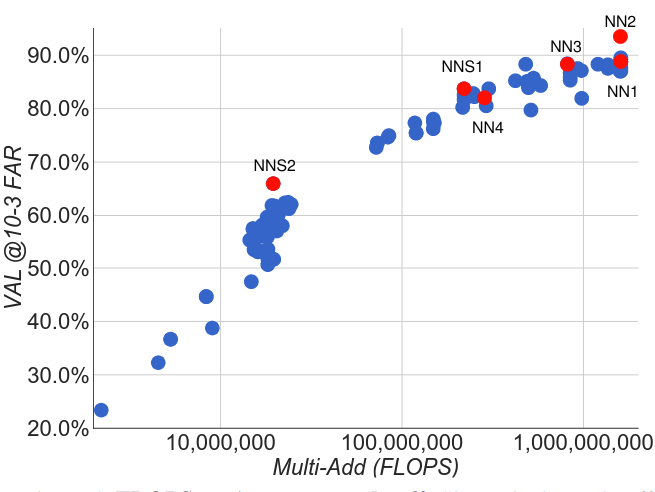
\includegraphics[width=.75\linewidth]{img/facenetflops}
	\caption{Porovnanie výpočtovej náročnosti v závislosti od úspešnosti siete, prebraté z\cite[s.~5]{schroff2015facenet}}
	\label{fig:facenetflops}
\end{figure}

\indent V ďalších čatiach si popíšeme konkrétnu implementáciu od Facenetu Sandberga \cite{davidsan26} pomocou knižnice Tensorflow v jazyku Python.

\subsection{Tensorflow}
Tensorflow je open source softvérová knižnica slúžiaca k náročným numerickým výpočtom, ako je napríklad strojové učenie.\cite{tensorflow2015}.
Jej implementácia dostupná na \url{https://github.com/tensorflow/tensorflow} umožňuje fungovanie na širokej škále systémov, nezávisle od operačného systému(Linux, Windows, Mac, Android ..), od hardvéru(umožňuje výpočty na jednom - viacerých CPU, jednom - viacerých GPU) a teda je použiteľná počnúc mobilnými zariadeniami až po veľké výpočtové strediská.
Podporuje veľké množstvo programovacích jazykov - Python, C++, Java, Go či najnovšie Javascript, vďaka čomu si zaslúžila obrovskú pozornosť verejnosti, a v súčastnosti je to najpopulárnejšia knižnica slúžiaca k učeniu hlbokých konvolučných sietí.\\

\indent Tensorflow je vyvíjaný spoločnosťou Google, pod Apache licenciou od roku 2015\cite{tensorflow2015}.
Jej fungovanie je postavené na využívaní grafových štruktúr a toku dát(data flow).
Uzly grafu reprezentujú vykonávané matematické operácie, premenné a konštanty, zatiaľ čo hrany reprezentujú dáta, ktoré sa presúvajú od jedného vrcholu k druhému.
Dáta sú reprezentované ako tensory, čo sú viac-dimenzionálne polia, z čoho vychádza aj samotný názov. \\

\indent Všetky výpočty v Tensorflowe sú reprezentované inštanciou triedy $ tf.Graph $. \cite{TensorFl6}
Graf pozostáva z inštancií tried $ tf.Tensor $ - dáta, a $ tf.Operation $ - napríklad maticové násobenie, špeciálneho typu uzlov - $ tf.Placeholder $ - ktoré reprezentujú uzly ktoré prijímajú dáta a $ tf.Variable $, ktoré uchovávajú hodnoty v grafe ktoré sa menia pri výpočte - napríklad hodnoty váh.
Je dôležité spomenúť, že graf definuje len samotnú štruktúru výpočtov, ale nie samotný výpočet.
Výpočet prebieha pomocou inštancie triedy $ tf.Session $. \\

\indent Na príklade z obrázku\ref{fig:tfexample} vidíme vytvorenie neurónovej siete slúžiacej na klasifikáciu ručne písaných čísel z datasetu MNIST, s jednou skrytou vrstvou, prijímajúcej dáta dáta o veľkosti 784(veľkosť snímku v MNIST datasete) do 10 tried.


\begin{lstlisting}[language=Python, label={fig:tfexample}, caption={Príklad klasifikácie pomocou Tensorflow}]
	# 1.Vytvor graf reprezentujci model.
	x = tf.placeholder(tf.float32, [BATCH_SIZE, 784])  # Miesto(placeholder) pre vstup.
	y = tf.placeholder(tf.float32, [BATCH_SIZE, 10])   # Placeholder pre triedy.
	
	W_1 = tf.Variable(tf.random_uniform([784, 100]))   # 784x100 matica vah.
	b_1 = tf.Variable(tf.zeros([100]))                 # 100-prvkovy bias vektor.
	layer_1 = tf.nn.relu(tf.matmul(x, W_1) + b_1)      # Vystup skrytej vrstvy.
	
	W_2 = tf.Variable(tf.random_uniform([100, 10]))    # 100x10 matica vah.
	b_2 = tf.Variable(tf.zeros([10]))                  # 10-element bias vector.
	layer_2 = tf.matmul(layer_1, W_2) + b_2            # Vystup linearnej vrstvy.
	
	# 2. Pridaj uzly reprezentujuce algoritmus minimalizacie chyby
	loss = tf.nn.softmax_cross_entropy_with_logits(layer_2, y)
	train_op = tf.train.AdagradOptimizer(0.01).minimize(loss)
	
	# 3. Spusti graph na davkach vstupnych dat
	with tf.Session() as sess:                         # Vytvorenie session.
	  sess.run(tf.initialize_all_variables())          # Inicializacia vah na nahodne hodnoty.
	  for step in range(NUM_STEPS):                    # Trenuj v cykle.
	    x_data, y_data = ...                           # Nacitaj davku vstupnych dat.
	    sess.run(train_op, {x: x_data, y: y_data})     # Vykonaj jeden treningovy cyklus.
\end{lstlisting}

\indent Knižnicu Tensoflow budeme používať pomocou jazyka Python pri trénovaní modelu a neskôr pomocou
jazyka Java, pri aplikácií modelu pod operačným systémom Android.

\subsection{Výber datasetu}
Pre trénovanie hlbokých neurónových sietí je potrebné použiť datasety, obsahujúce veľké množstvo trénovavích vzoriek.
Originálna Facenet implementácia \cite{schroff2015facenet} využíva tréningové datasety Labeled Faces in Wild(\acrshort{lfw}) a Youtube Faces.
Sandsbergova implementácia je trénovaná na datasetoch CASIA-WebFace a VGGFace2.
V pri našom finálnom trénovaní používame kombináciu LFW datasetu a zbierky osobných fotiek kvôli testovaniu na živých osobám na zariadení Android.

\subsubsection{Labeled Faces in Wild}
Tento datasaet obsahuje viac ako 13 000 obrázkov tvárí zozbieraných z webu.
V datasete sa nachádza približne 1700 ľudí, ktorý majú apsoň dve odlišné fotky tváre v datasete,
pričom každá tvár je priradená do priečinka s názvom nesúcim meno osoby na snímkoch\ref{fig:lfwf}.\cite{LFWTech}

\begin{figure}[H]
	\centering
	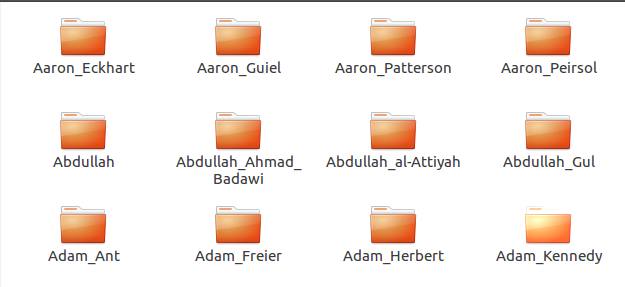
\includegraphics[width=0.5\linewidth]{img/lfwf}
	\caption{Štruktúra datasetu LFW}
	\label{fig:lfwf}
\end{figure}

\subsubsection{Youtube Faces}
Ide o dataset pozostávajúci z 3425 videí tvár prebratých z portálu Youtube, na ktorých sa nachádza 1595 rozličných ľudí, a teda priemerne 2.15 videa na jednu identitu.
Dĺžka videa sa pohybuje od 48 snímkov po 6070 s priemernou dĺžkou 181 snímkov.
Dataset je štruktúrou podobný LFW - a teda videá identít sa nachádzajú v priečinkoch nesúcich meno osoby na videu.\cite{wolf2011face}

\subsubsection{CASIA-WebFace}
Autori tohto datasetu uvádzajú, že v súčastnosti je v oblasti rozpoznávania tvárí pomocou konvolučných sietí dataset často dôležitejší, než samotný algoritmus\cite{Centerfo}.
Prichádzajú teda s riešením, v ktorom polo-automaticky zozbierali fotky tvárí z internetu a vytvorili databázu tvárí pozostávajúcu z 10 575 identít v celkovom počte 494 414 tvárí.
Po databáze tvárí Faceboooku(nie je verejne dostupná) a VGGFace2 ide o tretiu najväčšiu databázu tvárí.
\subsubsection{VGGFace2}
Ide v súčastnosti o najnovší veľký dataset tvárí, pozostávajúci z 3,31 milióna tvárí 9131 identít.
Tváre boli zozbierané pomocou Google Image Search, s veľkou variáciou v pózach, veku, osvetlení, etník či zamestnania.\cite{cao2017vggface2}
Ide teda o najväšiu voľne dostupnú databázu tvárí.

\subsection{Predspracovanie dát}
Trénovaniu modelu predbieha predspracovanie dát, najmä o odfiltrovanie niektorých nevhodných snímkov, detekciu tváre, jej zarovnanie či normalizácia.
Facenet \cite{davidsan26} pracuje s dvomi variantami pre detekciu tvárí:

\begin{itemize}
	\item Multi-task Cascade Convolutional Neural Networks(\acrshort{mtcnn})
	\item Dlib Face detector
\end{itemize}

\indent V tejto práci pracujeme s oboma možnosťami pre detekciu tvárí - MTCNN využívame pri trénovaní modelu a Dlib na zariadení Android.
V oboch prípadoch tváre škálujeme tvár do veľkosti $ 160 \times 160 $ s okrajom o veľkosti $ 25\% - 32px $.

\begin{lstlisting}[language=Bash, caption={Spustenie predspracovania tvárí pomocou MTCNN}]
for N in {1..4}; do python3 src/align/align_dataset_mtcnn.py ~/datasets/lfw/raw ~/datasets/lfw/alligned --image_size 160 --margin 32 --random_order --gpu_memory_fraction 0.25 & done~
\end{lstlisting}

\begin{lstlisting}[language=Bash, caption={Spustenie predspracovania tvárí pomocou Dlib}]
for N in {1..4}; do python3 tmp/align_dataset.py ~/datasets/lfw/raw ~/datasets/lfw/alligned_dlib --image_size 160 --margin 0.20 --dlib_face_predictor ~/models/dlib/shape_predictor_68_face_landmarks.dat & done
\end{lstlisting}

\indent Výsledné porovnanie snímkov pred a po detekovaní vidíme na obrázkoch\ref{fig:dlib_raw} a \ref{fig:dlib_aligned}.

\begin{figure}[H]
	\centering
	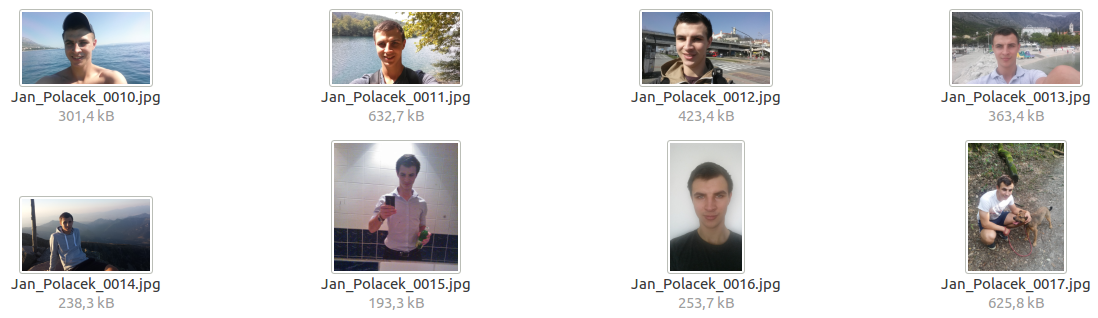
\includegraphics[width=1\linewidth]{img/dlib_raw}
	\caption{Fotky tvárí pred spracovaním}
	\label{fig:dlib_raw}
\end{figure}

\begin{figure}[H]
	\centering
	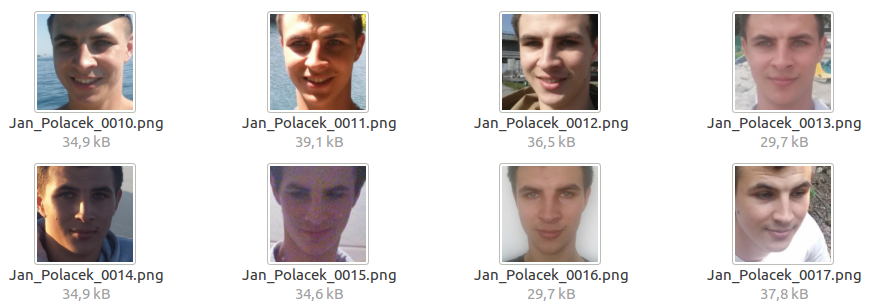
\includegraphics[width=1\linewidth]{img/dlib_aligned}
	\caption{Fotky tvárí po spracovaní}
	\label{fig:dlib_aligned}
\end{figure}


\subsubsection{MTCNN}
Najväčšou výhodou MTCNN je jeho presnosť pri detekcií tvárí v náročných podmienkach v porovnaní s Dlib, ktorý ich nebol schopný detegovať\cite{davidsan26}.
Tým bolo trénovanie siete výrazne uľahčené čo sa týka variácií póz a osvetlenia, čo v niektorých prípadoch zhoršilo výsledky pri finálnom rozpoznávaní tváre.
Z tohoto dôvodu bolo potrebné nájsť vhodnejší detektor tváre, ktorým bol zvolený MTCNN.\\

\indent Samotný detektor pozostáva z troch častí využívajúcich kaskádne konvolučné neurónové siete.
Prvá časť pozostáva z konvolučnej siete nazvanej Proposal Network(P-Net), ktorá slúži k získaniu  oblastí, ktoré sú kandidátom na výskit tváre a vektorov definujúcich ohraničenie týchto oblastí, podobným spôsobom ako v práci \cite{farfade2015multi}.
Následne sa použije algoritmus non-maximum supression na zlúčenie kandidátov, ktorý sa vo veľkej miere prekrývajú. \cite{mtcnn} \\

\indent V druhej fáze zavádzajú ďalšiu konvolučnú neurónovú sieť, nazvanú Refine Network(R-Net),
ktorá slúži k odfiltrovaniu veľkého množstva negatívnych kandidátov, vykoná kalibráciu ohraničení kandidátov a opäť zlúčenie kandidátov algoritmom non-maximum supression. \cite{mtcnn} \\

\indent Tretia fáza nazvaná The Output Network(O-Net) je podobná druhej, avšak viac sa zameriava na detailnejšie popísanie tváre, najmä o nájdenie dôležitých bodov tváre.\cite{mtcnn} \\

\indent Názornú ukážku ako každá z fáz funguje vidíme na obrázku\ref{fig:mtcnn}.

\begin{figure}[H]
	\centering
	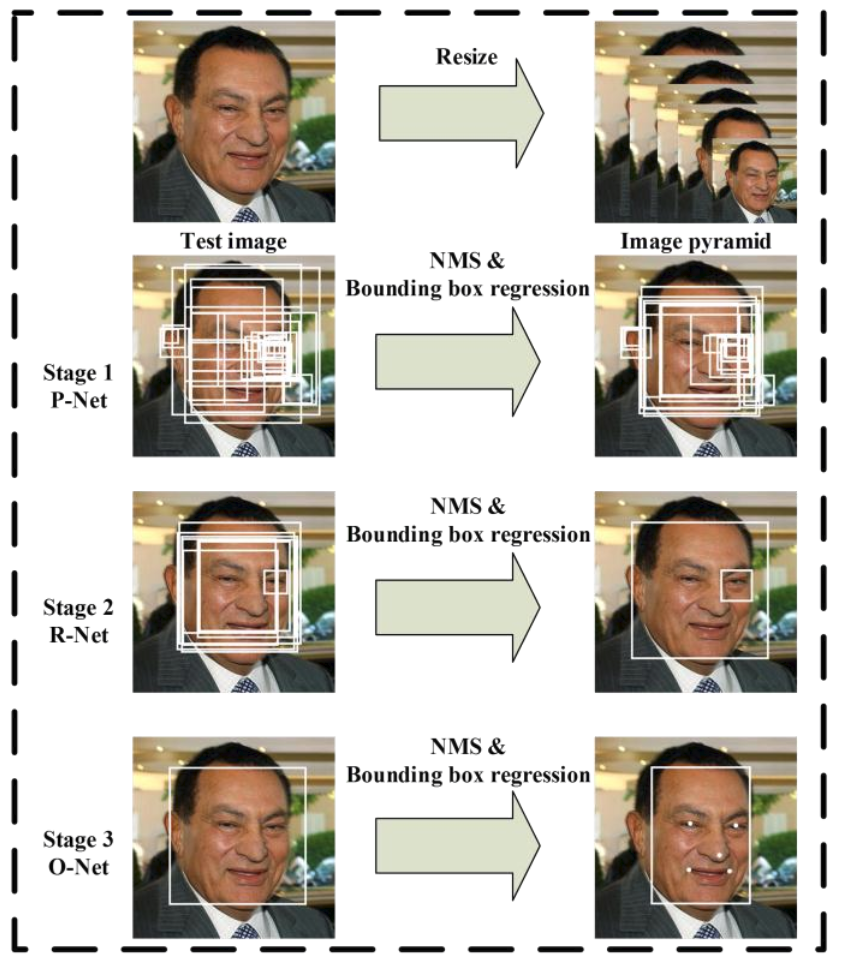
\includegraphics[width=0.6\linewidth]{img/mtcnn}
	\caption{Ukážka výsledkov každej z fáz MTCNN, prebraté z \cite[s.~2]{mtcnn}}
	\label{fig:mtcnn}
\end{figure}

\indent MTCNN dokáže spracovať snímky pri 16fps na procesore s výkonom 2.6Ghz, a 99fps na grafickej karte Nvidia Titan Black \cite{mtcnn}.
Tieto hodnoty nie sú problémom pri detekcií tvárí na silných počítačoch, avšak mobilné zariadenia nedisponujú možnosťou takýchto výpočtov na grafickom čipe, a taktiež procesor nemá dostatočný výkon aby bol schopný detegovať tvár v reálnom čase.
To je jedným z hlavných dôvodov, prečo MTCNN nepoužívame aj pri detekcií tvárí na zariadení Android, a namiesto toho využívame Dlib.

\subsubsection{Dlib}\label{l:dlib}
Dlib je open source knižnica napísaná v programovacom jazyku C++, obsahujúca algoritmy slúžiace k strojovému učeniu a jej pôvodným autorom je Davis King\cite{dlibCLib91}.
Má využitie v priemysle rovnako ako v akademickej sfére, a je možné ju použiť na širokom množstve zariadení, počnúc robotickými zariadeniami, mobilnými zariadeniami až po výkonné výpočtové centrá.
Medzi jej najväčšie výhody patrí výborná dokumentácia, portabilita a optimalizácie pre výpočty aj na mobilnom zariadení. \\

\indent Z tejto knižnice využijeme najmä predtrénovaný detektor tváre.
Knižnica taktiež ponúka dva natrénované modely detekcie bodov tváre - 5 - obrázok\ref{fig:dlib_5_landmarks} a 68 - obrázok\ref{fig:dlib_68_landmarks} bodový, na základe ktorých je potom možné vykonať zarovnanie tváre, ktorým docielime, že napríklad oči sa nachádzajú vo vodorovnej rovine v na približne rovnakej pozícii pre každú tvár.


\begin{figure}[H]
	\centering
	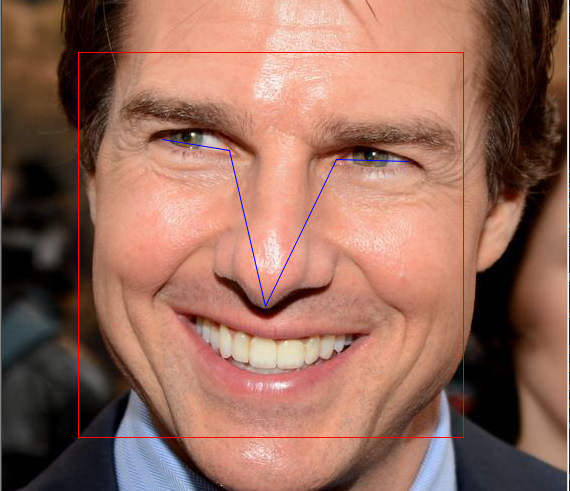
\includegraphics[width=.4\linewidth]{img/dlib_5_landmarks}
	\caption{Dlib - 5 bodová detekcia}
	\label{fig:dlib_5_landmarks}
\end{figure}


\begin{figure}[H]
	\centering
	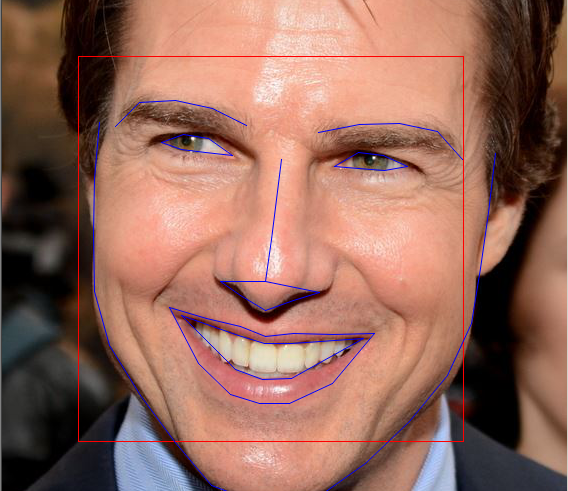
\includegraphics[width=.4\linewidth]{img/dlib_68_landmarks}
	\caption{Dlib - 68 bodová detekcia}
	\label{fig:dlib_68_landmarks}
\end{figure}

Model detektora je postavený na klasickom Histogram of Oriented Gradients(\acrshort{hog}) algoritme v kombinácií s lineárnym klasifikátorom, obrázkovou pyramídou(image pyramid) a schéme posúvajúceho sa okna.
Obrázkovou pyramídou myslíme postupnú zmenu veľkosti obrázka smerom hore alebo dole, v zmysle zmenšenia alebo zväčšia, ako na obrázku\ref{fig:pyramid}, kde vidíme 3 úrovne pyramídy. 

\begin{figure}[H]
	\centering
	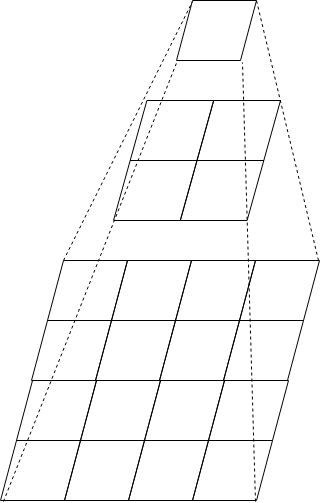
\includegraphics[width=.2\linewidth]{img/pyramid}
	\caption{Obrázková pyramída}
	\label{fig:pyramid}
\end{figure}

\subsubsection{Histogram of Oriented Gradients}
Ide o algoritmus slúžiaci primárne popisu príznakov pri detekcií objektov, založená na vyhodnocovaní dobre normalizovaných lokálnych histogramoch prechodov na pomyselnej mriežke na obrázku.
Základnou myšlienkou algoritmu, že objekty a ich tvár môžu byť často veľmi dobre popísané pomocou sily prechodov či orientácie hrán medzi oblasťami, aj bez znalosti presnej polohy prechodu či hrany.\cite{dalal2005histograms} \\


\indent Tento algoritmus pozostáva z rodelenia obrázka na malé oblasti označované ako bunky, a výpočtu 1-rozmerného histogramu gradientov prechodov a hrán pre každý pixel v bunke\cite{dalal2005histograms}.
Výpočet samotných gradientov pozostáva z aplikácie horizontálnej $ [-1, 0, 1] $ a vertikálnej $ [-1, 0, 1]^T $ derivačnej masky na obrázok.
Z nich je následne miera prechodu(gradient magnitude) rovnicou $ g = \sqrt{g_{x}^2 + g_{y}^2}$ \cite{Histogra74}.
Po vypočítaní miery prechodu je potrebné vypočítať orientáciu prechodu rovnicou $ \Phi = arctan\frac{g_{y}}{g_{x}}$.
Ich kombináciou získavame smer prechodu a jeho silu.

Celý algoritmus výpočtu HOG vidíme na obrázku\ref{fig:hog}

\begin{figure}[H]
	\centering
	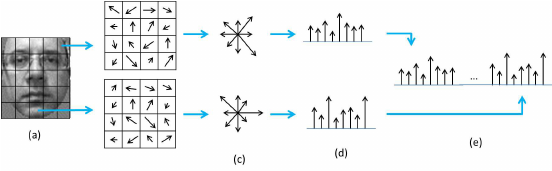
\includegraphics[width=1\linewidth]{img/hog}
	\caption{Algoritmus výpočtu HOG, prebraté z \cite{HOGextra27}}
	\label{fig:hog}
\end{figure}



\indent Skombinované histogramy všetkých oblastí potom tvoria reprezentáciu bloku.
Pre lepšiu invarianciu voči zmenám vo svetle či tieňom sa často aplikuje aj kontrastová normalizácia.
Posúvaním detekčného okna po mriežke sa zozbierajú vypočítané HOG do spoločného vektora príznakov, ktorý je následne použitý v klasickom SVM klasifikátore .
Celý proces trénovania HOG klasifikátora vidíme na obrázku\ref{fig:hog_class}.

\begin{figure}[H]
	\centering
	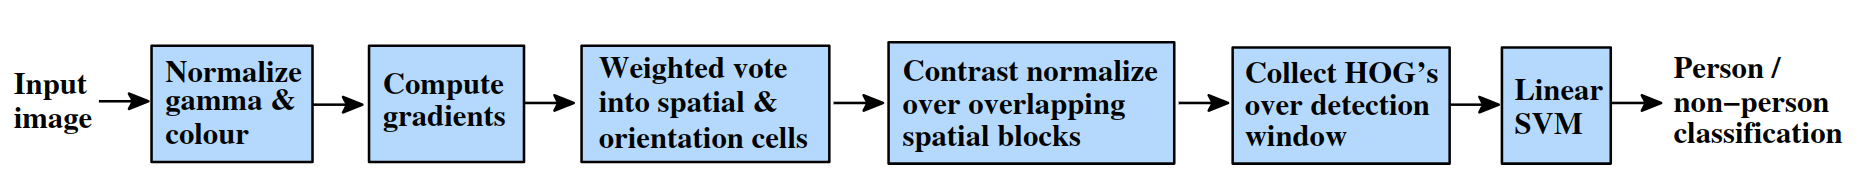
\includegraphics[width=1\linewidth]{img/hog_class}
	\caption{Diagram učenia HOG klasifikátora \cite[s.~3]{dalal2005histograms}}
	\label{fig:hog_class}
\end{figure}

\subsection{Klasifikovanie tváre}
Po fáze detekcie kedy sú snímky ľudí orezané a zarovnané, sa normalizujú do škály $ <-1, 1> $, algoritmom\ref{fig:prewhiten}.

\begin{lstlisting}[language=Python, label={fig:prewhiten}, caption={Normalizácia tváre}]
def prewhiten(x):
	mean = np.mean(x)
	std = np.std(x)
	std_adj = np.maximum(std, 1.0/np.sqrt(x.size))
	y = np.multiply(np.subtract(x, mean), 1/std_adj)
	return y
\end{lstlisting}

\indent Normalizované hodnoty vstupujú následne do natrénovaného Facenet modelu, ktorého výstupom je 128-rozmerný vektor príznakov pre každý zo snímkov z trénovacej množiny(v súčastnosti 512).
Tie sú následne použité v klasifikácií SVM ktoré sme popísali v\ref{svm} a natrénovaný model uložili.
Model sme trénovali na pri rôznych nastavenia minimálneho množstva snímkov ktoré musí mať identita a množstva trénovacích snímkov.
Prvým nastavením bolo použitie minimálne 40 snímkov pre osobu, čoho výsledkom bolo natrénovanie klasifikácie 21 tried, pozostávajúcich z datasetu LFW a 2 osôb z osobných zbierok autora.
Pri tomto nastavení bolo použitých 1261 snímkov v rozdelení $ 65\% $ trénovacích a $ 35\% $ testovacích s dosiahnutou úspešnosťou $ 99,4\% $.
Ďalším testovaním sme znižovali nároky na množstvo fotiek, ktoré musí mať identita, až po prípad kedy sme použili identity s minimálnym počtom snímkov 7 - a teda klasifikáciou do 250 tried, kde sme dosiahli úspešnosť $ 98,7\% $, čím sa potvrdila výborná kvalita natrénovaného extractora príznakov - Facenetu.
Výsledky testovania je možné vidieť na obrázku\ref{fig:chart}.

\begin{figure}[H]
	\centering
	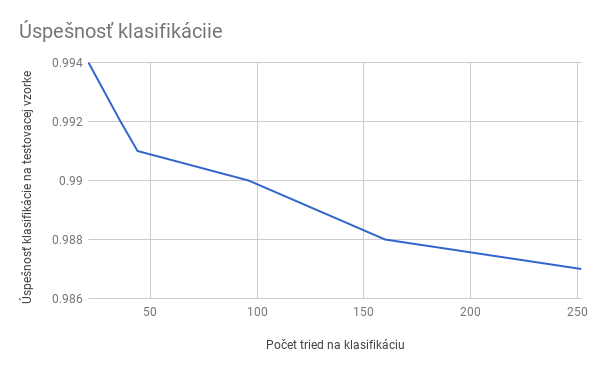
\includegraphics[width=1\linewidth]{img/chart}
	\caption{Výsledky testovania klasifikátora pri rôznych nastaveniach}
	\label{fig:chart}
\end{figure}

\indent Oproti pôvodnej Sandbergovej implementácii Facenetu sme v našej implementácii použili SVM klasifikátor z knižnice OpenCV, ktorá je na rozdiel od pôvodnej implementácie z knižnice Scipy, dostupná aj pre Android.


\subsection{Optimalizácia modelu}\label{l:opt}
Facenet bol v pôvodnom článku \cite{schroff2015facenet} trénovaný na architektúrach neurónových sietí typu Inception, konkrétna Sandbergova implementácia využíva model Inception-Resnet popísanej v \cite{SzegedyIV16}, vďaka ktorým dosahuje výborné výsledky čo sa týka chyby ktorú schopné dosiahnuť a rovnako aj rýchlosti učenia(learning rate).
Výsledky \cite{canziani2016analysis} však potvrdzujú aj náročnosť týchto sietí, kde trvanie za ktoré je sieť schopná vrátiť výsledok(inference time), sa pohybuje od 100 do 200ms na zariadení Nvidia TX1
Problémom nie je len náročnosť výpočtov, ale rovnako aj veľkosť samotného modelu - 93,3Mb.
Z týchto dôvodov je potrebné vykonať optimalizácie modelu tak, aby fungovali čo najlepšie na mobilnom zariadení. \\

\indent Autori Tensorflow poskytli príručku\cite{Optimizi3}, v ktorej navrhujú možné riešenia vedúce k optimalizácií modelov neurónových sietí a taktiež k nej viazané nástroje.
Prvým krokom je výpočet našej optimalizácie je odhad náročnosti modelu(Facenet), ktorý sa bude používať.
Naše referenčné zariadenie, ktoré budeme používať je Samsung Note3, ktorý má výkon približne 5BFLOPS. 

\begin{lstlisting}[language=Bash, label={fig:optim}, caption={Spustenie procesu analýzy modelu}]
bazel-bin/tensorflow/tools/benchmark/benchmark_model  --graph=/home/jan/models/facenet/20170512-110547.pb  --input_layer="input:0,phase_train,batch_size"  --input_layer_shape="1,160,160,3::1"  --input_layer_type="float,bool,int32"  --output_layer="embeddings:0"  --show_run_order=false  --show_time=false  --show_memory=false  --show_summary=true  --show_flops=true
\end{lstlisting}


\indent Spustením príkazu\ref{fig:optim}, dostávame sériu štatistických informácií o tom, koľko každý uzol modelu vyžaduje času či jeho výpočtovú náročnosť.
Z nich za najsmerodajnejšie považujeme výsledky\ref{fig:optim_res}, kde vidíme, že priemerný čas inferencie je 0,605 sekundy a náročnosť modelu 2.83BFLOPS.

\begin{lstlisting}[language=Bash, label={fig:optim_res}, caption={Výsledky analýzy modelu}]
Timings (microseconds): count=32 first=1174163 curr=569701 min=479800 max=1174163 avg=605828 std=138948
Memory (bytes): count=32 first=38866348 curr=38910508 min=38824236 max=39015084 avg=3.89352e+07 std=46903
4349 nodes observed
FLOPs estimate: 2.83B
\end{lstlisting}

\indent Jedným z možných riešení je použitie nástrojov, ktoré umožňujú spojenie uzlov v grafe modelu, a odstránenie uzlov, ktoré boli napríklad potrebné len v procese trénovania, ale pri aplikácii sa nepoužívajú.
Ich použitím sme dosiahli výsledky\ref{fig:optim_res_f}, na ktorých vidíme 100ms zlepšenie výkonu modelu,teda približne o $ 15\% $.
Oveľa markantnejším výsledkom je však zredukovanie veľkosti modelu, ktorú sa podarilo zredukovať na $ 25,2Mb $, teda približne o $ 73\%  $

\begin{lstlisting}[language=Bash, label={fig:optim_res_f}, caption={Výsledky analýzy modelu po optimalizácii}]
Timings (microseconds): count=38 first=505042 curr=476550 min=473424 max=676329 avg=506505 std=34466
Memory (bytes): count=38 first=38878380 curr=38921388 min=38849964 max=39028268 avg=3.89496e+07 std=47100
4349 nodes observed
FLOPs estimate: 2.83B
\end{lstlisting}

\indent V súčastnosti prebieha ďalší výskum v oblasti optimalizácie modelov neurónových sietí a ich aplikácia na mobilných zariadeniach, ako napríklad SqueezeNet\cite{IandolaMAHDK16}, kde sa podarilo zmenšenie modelu siete AlexNet o viac ako $ 50 \times $, či výskum MobileNet \cite{HowardZCKWWAA17}, ktorý je v súčastnosti vyvíjaný ako súčasť knižnice Tensorflow. 
Celý workflow trénovania modelu je zobrazený na obrázku\ref{fig:trainig_workflow}.

\begin{figure}[H]
	\centering
	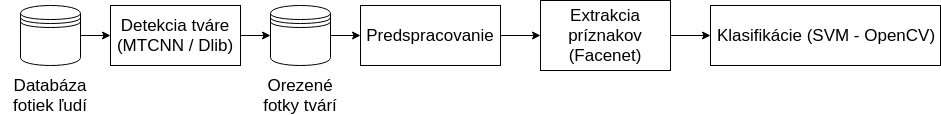
\includegraphics[width=1\linewidth]{img/trainig_workflow}
	\caption{Worfklow trénovania modelu}
	\label{fig:trainig_workflow}
\end{figure}

\newpage 

\section{Rospoznávanie tvárí na zariadení Android}\label{l:andapp}
Cieľom tejto práce je aplikovať natrénovaný model konvolučnej siete pri rozpoznávaní tváre na zariadení Android.
V prechádzajúcich častiach práce sme popísali časť detekcie tváre, model, ktorý budeme používať na extrahovanie príznakov tváre - Facenet, spôsob klasifikácie extrahovaných príznakov a nakoniec optimalizáciu modelu.
Poslednou fázou je samotné použitie modelu na zariadení Android.
Workflow fungovania samotnej aplikácie je podobný ako na obrázku\ref{fig:trainig_workflow}, rozdielom je zdroj dát, ktorým je v našom prípade živá kamera.
V nasledujúcich sekciách popíšeme operačný systém Android, niektoré jeho súčasti, ktoré využívame a najmä samotnú funkcionalitu aplikácie, ktorú sme nazvali Face classifier.

\subsection{Android OS}
Android je operačný systém pre mobilné zariadenia, vyvíjaný spoločnosťou Google a je postavený na upravenej verzií linuxového jadra.
Aplikácie sú vyvíjané používaním Android Sofware Development Kit-u(\acrshort{sdk}), najčastejšie v programovacom jazyku Java alebo Kotline, a vďaka rozšíreniu - Native Development Kit(\acrshort{ndk}) taktiež podporuje písanie kódu v jazykoch C/C++ \cite{Applicat21}.
Podobne ako Java aplikácie, aj Android aplikácie bežia každý vo vlastnom virtuálnom stroji, izolovaný od ostatných aplikácií.
Android funguje na princípe najmenšieho množstva oprávnení, takže pri inštalácií alebo spustení aplikácia vyžaduje povolenia, ktoré jej buď udelíme, alebo zakážeme, za cenu obmedzenej funkcionality. \\

\indent Aplikácie sa vytvárajú skladaním základných komponentov, ktorými systém alebo užívateľ môže pristúpiť k aplikácii:
\begin{itemize}
	\item Aktivity (Activities)
	\item Služby (Services)
	\item Prijímače vysielania (Broadcast receivers)
	\item Poskytovatelia obsahu (Content providers)
\end{itemize}
\cite{Applicat21}

\indent Z týchto komponentov využíva Face classifier iba Aktivity.
Aktivita je vstupným bodov slúžiacim na interakciu s užívateľom.
Je reprezentovaná jedinou obrazovkou s užívateľským prostredím - v našom prípade ide o zobrazenie obrazu z kamery. 
Aplikácia môže obsahovať jednu ale aj viacero aktivít, pričom v jednom okamihu môže mať aplikácia spustenú práve jednu.
Životný cyklus aktivity začína metódou onCreate, a končí onDestroy, pričom medzi nimi môžu byť spustené aj iné - onStart, onResume, onPause, onStop, v závislosti od momentálneho stavu aktivity a aplikácie.
Celý životný cyklus aplikácie je popísaný diagramom 
\begin{figure}[H]
	\centering
	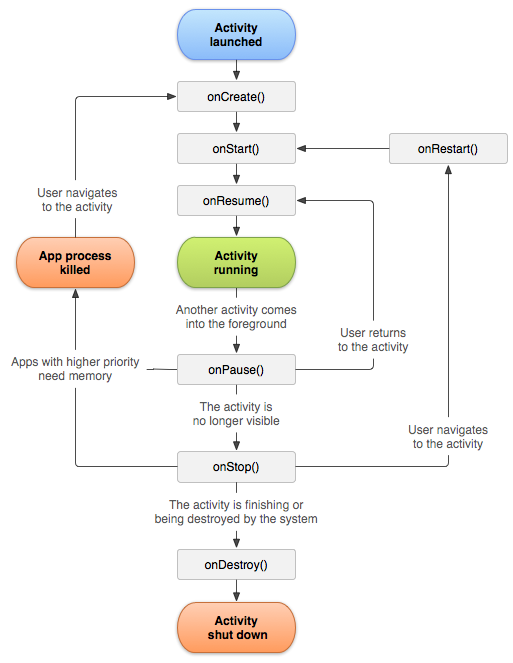
\includegraphics[width=.5\linewidth]{img/activity_lifecycle}
	\caption{Zjednodušený diagram životného cyklu aktivity, prebraté z \cite{Understa46}}
	\label{fig:activity_lifecycle}
\end{figure}

\subsection{Spracovanie obrazu z kamery}
Ako sme uz spomenuli, Face classifier pozostáva z jedinej aktivity, na ktorej zobrazujeme obraz snímaný kamerou, na ktorý vykresľujeme ohraničenie detekovanej a klasifikovanej tváre.
Aplikácia vyžaduje 2 špeciálne povolenia k správnemu fungovaniu - povolenie k používaniu kamery a čítanie a zápis na zariadenie.
Povolením oboch začína naša aplikácia fungovať. \\

\indent Na spracovanie obrazu z kamery využívame knižnicu Fotoapparat.
Nahradili sme ňou našu pôvodnú implementáciu používania kamery, ktorá nepokrývala všetky hraničné prípady vychádzajúce zo životného cyklu aktivity a tiež nebola taká flexibilná čo sa týka užívateľských nastavení.
Fotoapparat podporuje API fotoaparátu rovnako starších verzií Androidu aj nových,
opravuje chyby špecifické pre niektoré zariadenia, rôzne užívateľské nastavenia - napríklad. veľkosť obrazu, výber kamery a najmä ponúka jednoduché riešenie pre spracovanie hrubého(raw) obrazu z kamery prostredníctvom triedy $ FrameProcessor $ a implementácie metódy $ process $ \cite{Fotoappa49}. \\

\indent Aplikácia využíva 2 vlákna - v hlavnom sa zobrazuje obraz kamery, zatiaľ čo v druhom prebiehajú náročnejšie výpočty ako detekcia a klasifikácia.
Veľkosť snímkov je maximálna akú zariadenie podporuje, a to v prípade Samsung Note 3 $ 1920 \times 1080  $.
Pre každý snímok z kamery je spustená metóda $ process $, ktorej vstupným argumentom je snímok v kódovaní farieb YUV NV21 \cite{YUVWikip53}.
Ten odosielame do detektora tváre, spolu s informáciou o rozmeroch a rotácií snímku.

\subsection{Detekcia tváre}
Ako detektor tváre využívame Dlib, ktorý sme popísali už v časti\ref{l:dlib}.
Jeho výhodou je implementácia dostupná v C++, rýchlosť a presnosť detekcie v porovnaní s existujúcimi riešeniami a taktiež podpora procesorových inštrukcií SSE2, SSE4 a AVX, vedúcich k optimálnejšiemu výkonu.
Problémom bola chýbajúca implementácia pre mobilné zariadenia Android, umožňujúca volanie C++ kódu z Javy, ktorú sme museli vytvoriť.
Inšpirovali sme sa pri tom implementáciou \cite{tzutalin82}, ktorá je však zastaraná a nepodporuje novšie verzie Dlib a Android NDK. \\

\indent Implementácia v C++ bola kľúčová z dôvodu oveľa rýchlejšieho spracovania v porovnaní s jazykom Java.
Volanie C++ prebieha prostredníctvom Java Native Interface(\acrshort{jni}), ktoré umožňuje vytváranie inštancií Java tried, volanie Java metód, používať a zachytávať výnimky či načítavať triedy a informácie o nich \cite{Introduc22}. \\

\indent Samotný detektor je inicializovaný len jediný krát - pri spustení aplikácie a potom žije v pamäti, kedy zároveň načíta model slúžiaci k lokalizácii bodov tváre.
Pri implementácii aplikácie sme testovali oba z natrénovaných modelov (5 a 68 bodový) bez výraznejšieho rozdielu v zarovnaní tváre alebo rýchlosti lokalizácie bodov.
Vo finálnom riešení sme sa rozhodli pre 5 bodový detektor, najmä z dôvodu menšej 9Mb veľkosti v porovnaní s 99Mb, ktorú má 68 bodový. \\

\indent Detekcia tváre začína transformáciou farebnej škály snímku do RGB a jeho rotovaním.
Z originálneho snímku vytvárame čiernobielu kópiu, ktorú následne 4 násobne zmenšíme.
Štvornásobné zmenšenie sa ukazuje byť adekvátnym pre toto riešenie, pretože veľkosť snímku stále umožňuje detekciu tváre a jej polohy na niekoľko metrov a zároveň urýchľuje proces detekcie tváre.
V prípade prítomnosti tváre spätne prepočítame jej polohu na originálnom snímku, 
z ktorého tvár vystrihneme (chips), a na základe bodov tváre (oči) zarovnáme a zmenšíme na veľkosť, podobne ako pri fáze trénovania - $ 160 \times 160 pixelov $.
Normalizované tváre vraciame späť do Javy, prostredníctvom vytvorenia inštancií tried $ Detection $, a naplnenia jej hodnôt orezanou tvárou a polohou.
Na základe polohy snímku následne na obrazovku vykresľujeme štvorec ohraničujúci tvár. \\

\indent Celý proces detekcie tváre trvá približne 120ms + 25ms pre káždú detekovanú tvár. 
Pri implementácií aplikácie sa nám podarilo vytvoriť optimálnejšie riešenie na detekciu jednej tváre, v ktorom trvala detekcia 70ms.
Dlhšia detekcia tváre vnikla rozšírením funkcionality aplikácie na detekciu viacerých tvárí, v kombinácií s pridaným zachovávaním originálneho RGB snímku, slúžiacemu k deterministickejšiemu porovnaniu výsledkov detektora.
Ukážku výsledku fázy detekcie vidíme v podobe štvorcov na obrázku\ref{fig:android_dlib}.
\begin{figure}[H]
	\centering
	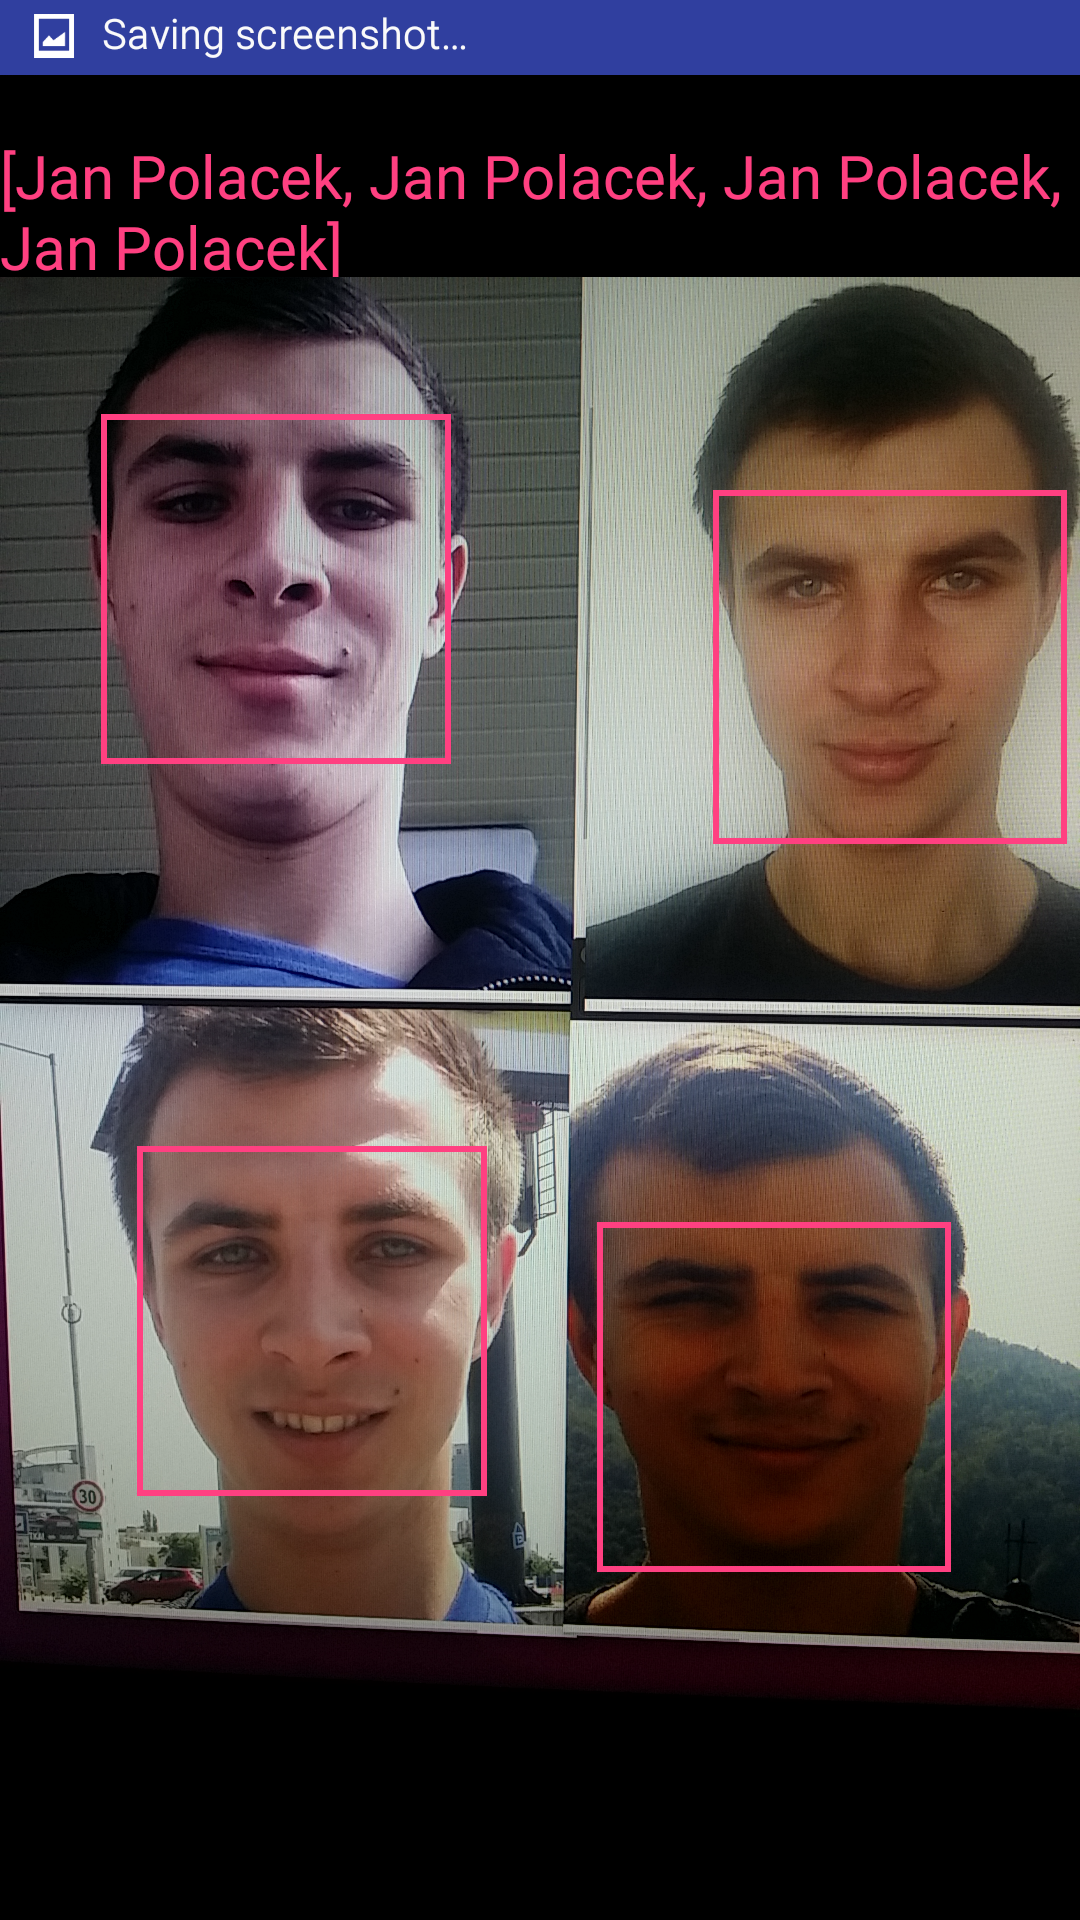
\includegraphics[width=.5\linewidth]{img/android_dlib}
	\caption{Lokalizácia pozícií tvárí na Androide použítím knižnice Dlib}
	\label{fig:android_dlib}
\end{figure}

\indent Ako sme spomenuli v prechádzajúcej kapitole, detektor knižnice Dlib má niekedy problém s detekciou, najmä v zhoršených podmienkach.
Riešením sa javí MTCNN, čo je však konvolučná neurónová sieť, v prípade ktorej by mohlo dôjsť k zhoršeniu výkonu aplikácie.
Ďalším možným zlepšením výkonu pri detekcií tváre by mohlo byť sledovanie pohybu, podobne ako to robí ROLO detektor\cite{redmon2016you}. \\

\indent Po úspešnom detekovaní tvárí zavoláme post funkciu ovládača hlavného vlákna, slúžiaci k vykresleniu štvorcov, a pokračujeme fázou extrahovania príznakov vo vedľajšom vlákne.

\subsection{Extrahovanie príznakov}
Extrahovanie príznakov prebieha obdobým spôsobom ako v prípade trénovania klasifikátora.
Využívame k nemu Tensorflow a jeho interface, slúžiaci k volaniu C++ funkcí cez JNI.
Proces začína načítaním, inicializáciou natrénovaného Facenet modelu z uložiska zariadenia a nájdením vstupných a výstupných uzlov grafu modelu (input, embedding).
Dáta z fázy detekcie normalizujeme funkciou ekvivalentnou s algoritmom\ref{fig:prewhiten}, a transformujeme na jednorozmerné pole, ktoré má následne veľkosť $ počet detekcií * výška obrázka * šírka obrázka * počet kanálou$.
Takýto vektor odošleme ako parameter funkcie interfacu Tensorflow - feed, slúžiacej k inicializácii hodnôt uzlov grafu, následne metódu run ktorej parametrom je názov uzla, z ktorého chceme získať výsledok a nakoniec metódu fetch, ktorá slúži k samotnému získaniu hodnôt uzla, viď obrázok\ref{fig:tfjavaexample}.

\begin{lstlisting}[language=Java, label={fig:tfjavaexample}, caption={Extrakcia príznakov pomocou Facenet na zariadení Android}]
inferenceInterface.feed(inputName, mats, detections.size(), inputSize, inputSize, 3);
inferenceInterface.feed("phase_train", false);
inferenceInterface.run(outputNames, false);
inferenceInterface.fetch(outputName, output);
\end{lstlisting}

\indent Fáza extrahovania trvá podľa predpokladov z analýzy modelu približne 500ms pre extrahovanie príznakov z jedného snímku.

\subsection{Klasifikácia tváre}
Klasifikácia tváre je finálnou časťou procesu spracovania snímku.
Táto fáza pozostáva z načítania natrénovaného modelu SVM klasifikátora z knižnice OpenCV a označení tried (mená ľudí), a samotnej klasifikácie.
Táto časť trvá najkratšie, približne len 1ms, a výsledkom klasifikácie sú identifikátory klasifikovaných tried, ktoré sú následne nahradené skutočnými menami ľudí, obrázok \ref{fig:android_dlib}.

\indent Zjednodušený diagram fungovania aplikácie je možné vidieť na obrázku\ref{fig:android}
\begin{figure}[H]
	\centering
	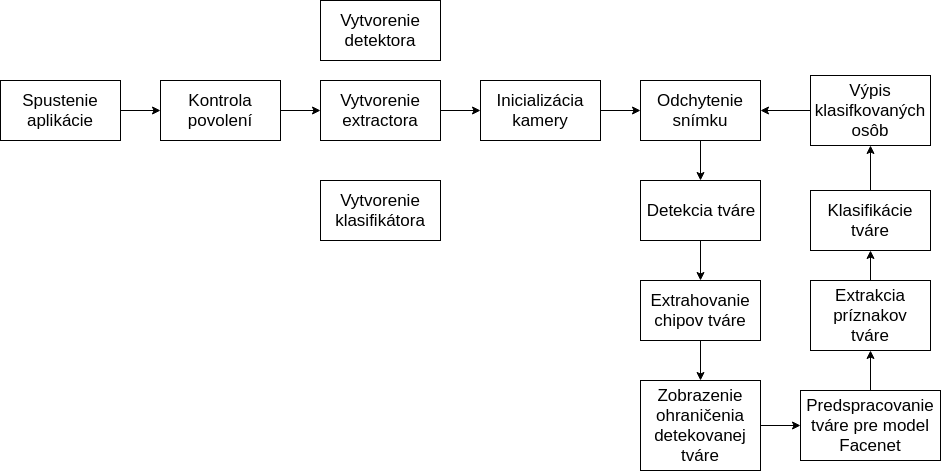
\includegraphics[width=1\linewidth]{img/android}
	\caption{Schéma fungovania aplikácie}
	\label{fig:android}
\end{figure}

\indent Klasifikátor priradí príznakom najpodobnejšiu identitu, avšak použitím SVM klasifikátora z OpenCV neumožňuje určiť pravdepodobnosť správneho určenia triedy, ako napríklad v prípade lineárneho klasifikátora.
Výsledkom je teda priradenie nesprávnej identity v prípade neznámej tváre.
